\documentclass[a4paper,12pt,twoside]{article}
\usepackage[utf8]{inputenc}
\usepackage{graphicx}
\usepackage{float}
\usepackage[brazilian]{babel}
\usepackage{indentfirst}
\usepackage{steinmetz}
\usepackage[left=2cm, right=2cm, top=2cm]{geometry}
\setlength\parindent{1cm}
\usepackage{mathrsfs, amsmath}
\usepackage{textcomp}
\usepackage{gensymb}
\usepackage{lipsum}




\headheight = 10pt

\setcounter{section}{-1}

\begin{titlepage}
\begin{center}
{\large Universidade Federal do Rio de Janeiro}\\[0.2cm]
{\large Engenharia Eletrônica e de Computação}\\[0.2cm]
{\large Trabalho de Sistemas Lineares 1}\\[5.1cm]
{\bf \huge GRUPO 11}\\[5.1cm]
\end{center}
{\large Alunos(as): Catarina Dowsley, Gabriel de Lima e Karen Arcoverde}\\[0.7cm]
{\large Professor: Jomar Gozzi}\\[5.1cm]
\begin{center}
{\large Rio de Janeiro}\\[0.2cm]
{\large 2019.1}
\end{center}
\end{titlepage}


\begin{document}

\tableofcontents
\maketitle

\section{Introdução}

 Nesse trabalho, iremos analisar o modelo linear de um sistema dinâmico representado pela função de transferência relacionando a entrada f(t) e a saída y(t), dada como:

\begin{equation} \\ \label{eqfunction}
H(s)={\frac{\alpha}{s^3 +4s^2 +3s +\alpha}}
\end{equation}



%%%%%%%%%%%%%%%%%%%%%%%%%%% SEÇÂO 1 %%%%%%%%%%%%%%%%%%%%%%%%%%%%%%%
\section{Resposta analítica ao degrau unitário}

%%%%%%%%%%%%%%%%%%%%%%%%%%% Análise das Raízes
\subsection{Análise das raízes}

Primeiramente vamos analisar os pólos da função de transferência em função do parâmetro $\alpha$. Para encontrar as raízes dessa função podemos utilizar a equação cúbica:\\
Sabendo que a equação cúbica é da forma:
$as^3 +bs^2 +cs + d = 0$

\begin{equation}
r_{1} = -\frac{b}{3a} +\sqrt[3]{\frac{-q}{2} + \sqrt{\frac{q^2}{4} +\frac{p^3}{27}}} +\sqrt[3]{\frac{-q}{2} -\sqrt{\frac{q^2}{4}+\frac{p^3}{27}}}
\end{equation}
\begin{equation}
r_{2} = -\frac{b}{3a} (-\frac{1}{2} +\frac{j\sqrt{3}}{2})\sqrt[3]{\frac{-q}{2} + \sqrt{\frac{q^2}{4} +\frac{p^3}{27}}} (-\frac{1}{2} -\frac{j\sqrt{3}}{2})\sqrt[3]{\frac{-q}{2} -\sqrt{\frac{q^2}{4}+\frac{p^3}{27}}}
\end{equation}
\\
\begin{equation}
r_{3} = -\frac{b}{3a} (-\frac{1}{2} -\frac{j\sqrt{3}}{2})\sqrt[3]{\frac{-q}{2} + \sqrt{\frac{q^2}{4} +\frac{p^3}{27}}} (-\frac{1}{2} +\frac{j\sqrt{3}}{2})\sqrt[3]{\frac{-q}{2} -\sqrt{\frac{q^2}{4}+\frac{p^3}{27}}}
\end{equation}
em que:
\begin{equation}
p = \frac{c}{a}-\frac{b^2}{3 a^2}\end{equation}
\begin{equation}
q = \frac{d}{a} -\frac{bc}{3a^2} +\frac{2b^3}{27a^3}
\end{equation}
\\
\\
Substituindo a = 1, b = 4, c = 3 e d = $\alpha$ e manipulando as expressões:
\\
\\
Raíz  1: 
\begin{align} \label{r1} 
r_{1} = \frac{7}{9\sqrt[3]{\sqrt{(\frac{\alpha}{2}+\frac{10}{27})^2 -\frac{243}{729}}-\frac{\alpha}{2}-\frac{10}{27}}}+\sqrt[3]{\sqrt{(\frac{\alpha}{2}+\frac{10}{27})^2-\frac{243}{729})}-\frac{\alpha}{2}-\frac{10}{27}}-\frac{4}{3}
\end{align}
\\
Raíz  2:
\begin{align*} \label{r2}
r_{2} = -\frac{\sqrt{3}\sqrt[3]{\frac{7}{9\sqrt[3]{\sqrt{(\frac{\alpha}{2} + \frac{10}{27})^2 - \frac{343}{279}}-\frac{\alpha}{2}-\frac{10}{27}}}-\sqrt[3]{\sqrt{(\frac{\alpha}{2} + \frac{10}{27})^2 - \frac{343}{279}}-\frac{\alpha}{2}-\frac{10}{27}}}}{2}j
\end{align*}
\begin{align} 
-\frac{7}{18\sqrt[3]{\sqrt{(\frac{\alpha}{2} + \frac{10}{27})^2 - \frac{343}{279}}-\frac{\alpha}{2}-\frac{10}{27}}}-\frac{ \sqrt[3]{\sqrt{(\frac{\alpha}{2} + \frac{10}{27})^2 - \frac{343}{279}}-\frac{\alpha}{2}-\frac{10}{27}}  }{2}-\frac{4}{3}
 \end{align}
\\
Raíz  3: 
\begin{align*} \label{r3}
 r_{3} = \frac{\sqrt{3}\sqrt[3]{\frac{7}{9\sqrt[3]{\sqrt{(\frac{\alpha}{2} + \frac{10}{27})^2 - \frac{343}{279}}-\frac{\alpha}{2}-\frac{10}{27}}}-\sqrt[3]{\sqrt{(\frac{\alpha}{2} + \frac{10}{27})^2 - \frac{343}{279}}-\frac{\alpha}{2}-\frac{10}{27}}}}{2}j
 \end{align*}
 \begin{align}
 -\frac{7}{18\sqrt[3]{\sqrt{(\frac{\alpha}{2} + \frac{10}{27})^2 - \frac{343}{279}}-\frac{\alpha}{2}-\frac{10}{27}}}-\frac{ \sqrt[3]{\sqrt{(\frac{\alpha}{2} + \frac{10}{27})^2 - \frac{343}{279}}-\frac{\alpha}{2}-\frac{10}{27}}  }{2}-\frac{4}{3}
\end{align}

 Simulando no matlab ($\alpha > 0$) em um gráfico raiz x $\alpha$ encontramos:
\\


Raíz  1:
\begin{figure}[H]
\centering
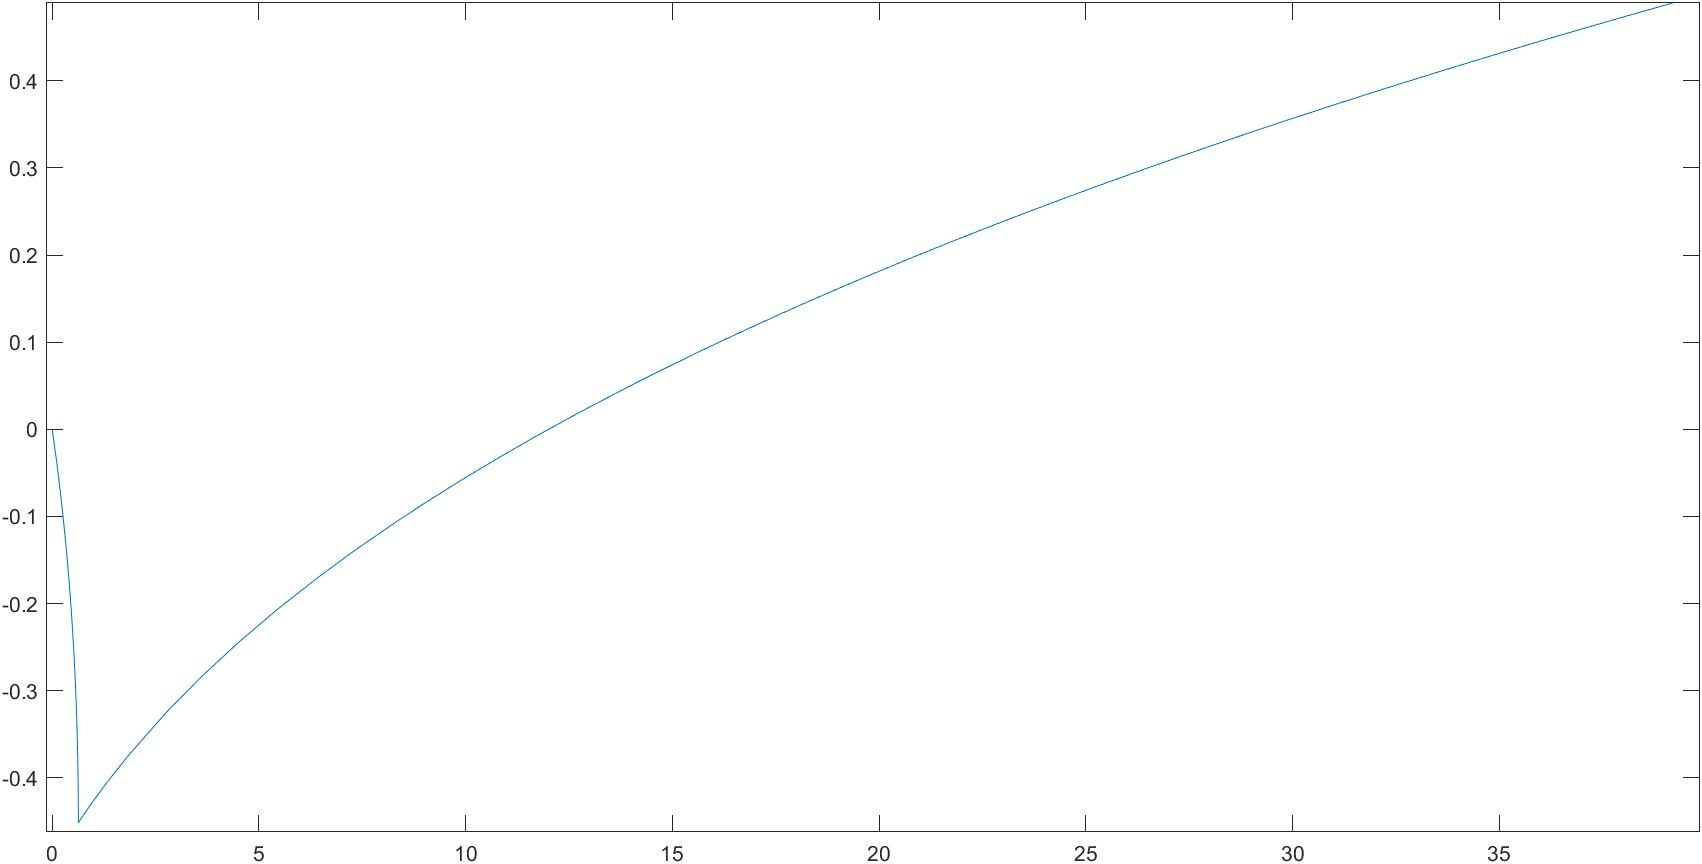
\includegraphics[scale=0.2]{real1.jpg}
\caption{Parte Real - Raíz 1}
\label{fig:real1}
\end{figure}
\begin{figure}[H]
\centering
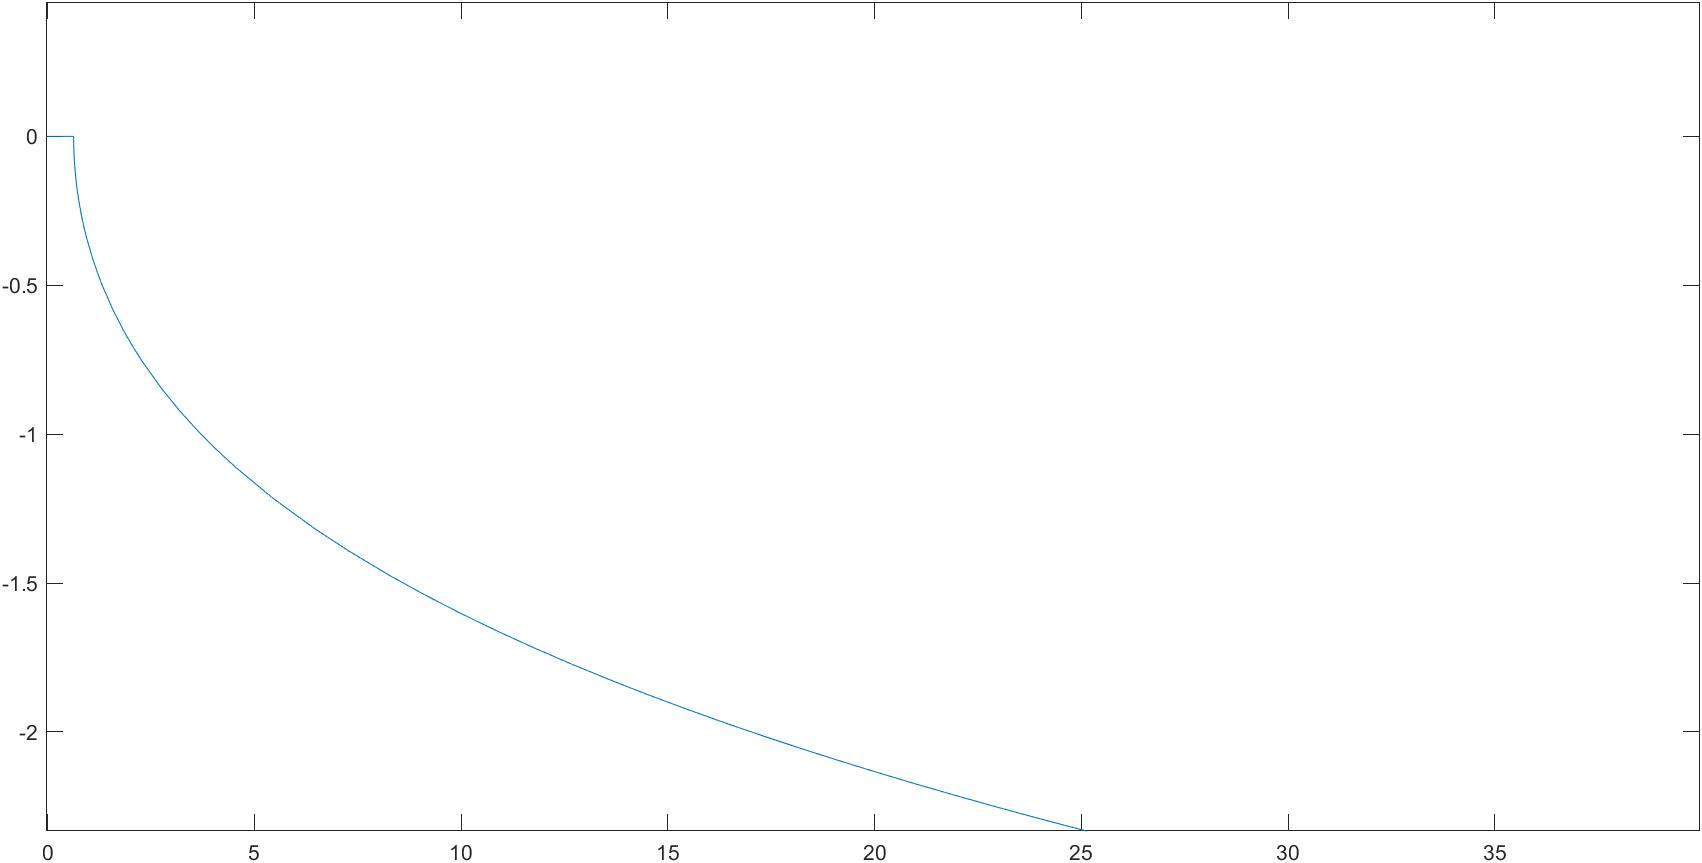
\includegraphics[scale=0.2]{img1.jpg}
\caption{Parte Imaginária - Raíz 1}
\label{fig:real1}
\end{figure}
Para a raíz 1 podemos tirar as seguintes conclusões:
A parte imaginária será sempre negativa para $\alpha>0$.Para $0<\alpha<12$ a parte real será negativa, para $\alpha=12$ ela será zero e para $\alpha>12$ ela será positiva. Então, concluímos que a raiz 1 quando $t\rightarrow \infty$, de $0<\alpha<12$ contribuirá para a resposta com uma senoide que tende a zero. Além disso, $\alpha=12$, será uma senoide que oscila sem tender a infinito e a zero. Já para $\alpha>12$, será uma senoide que oscila tendendo a infinito.
\\
\\
Raíz  2:
\begin{figure}[H]
\centering
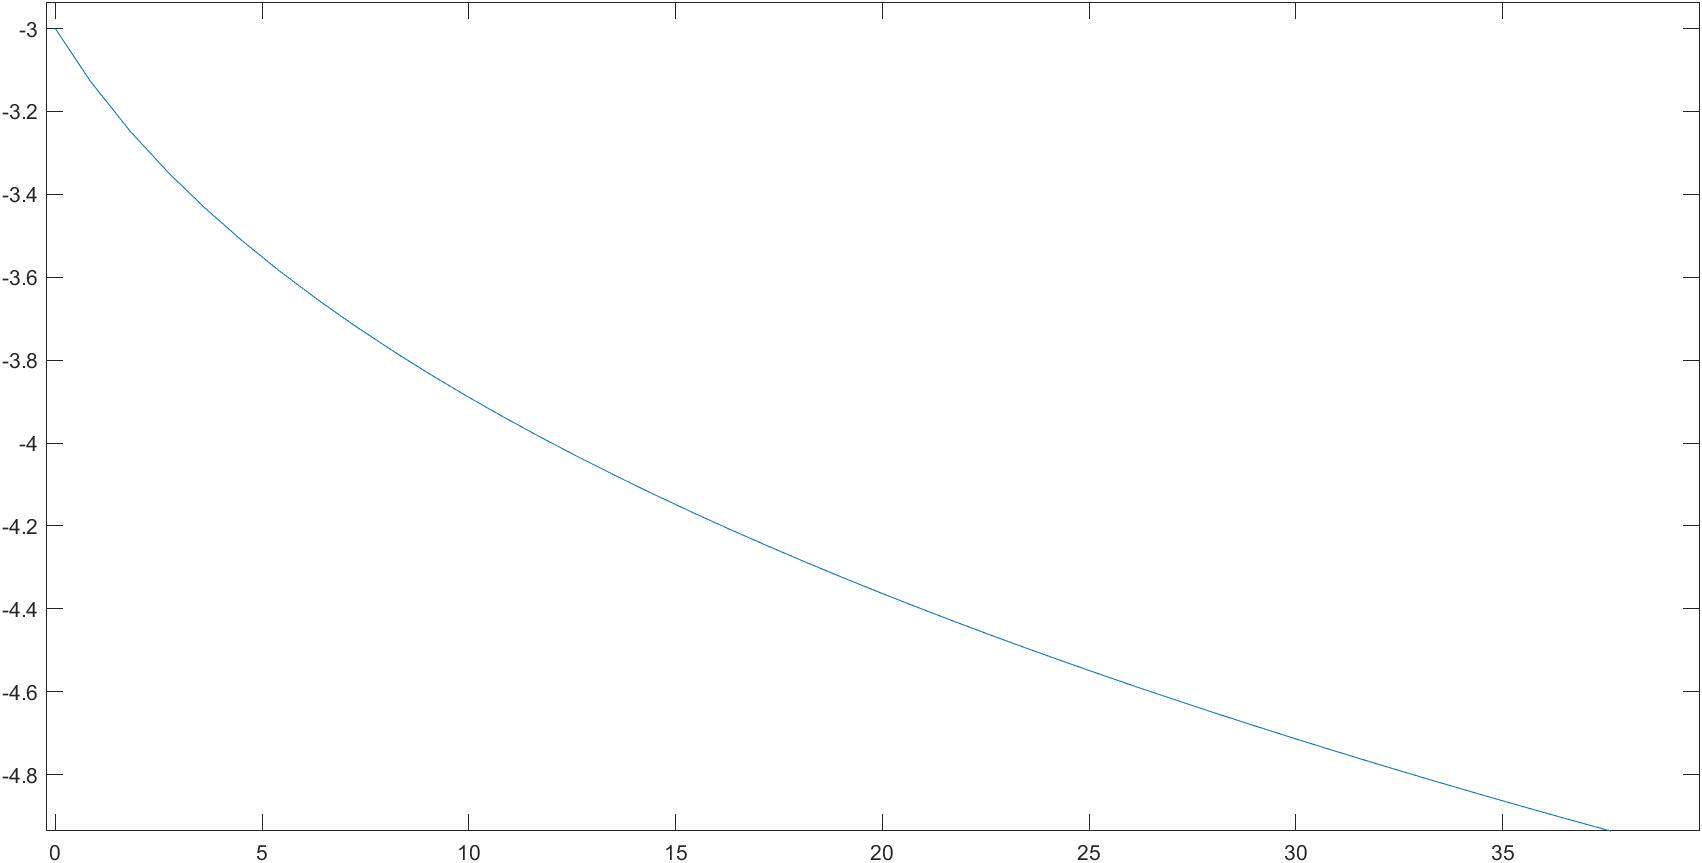
\includegraphics[scale=0.2]{real2.jpg}
\caption{Parte Real - Raíz 2}
\label{fig:real2}
\end{figure}
\begin{figure}[H]
\centering
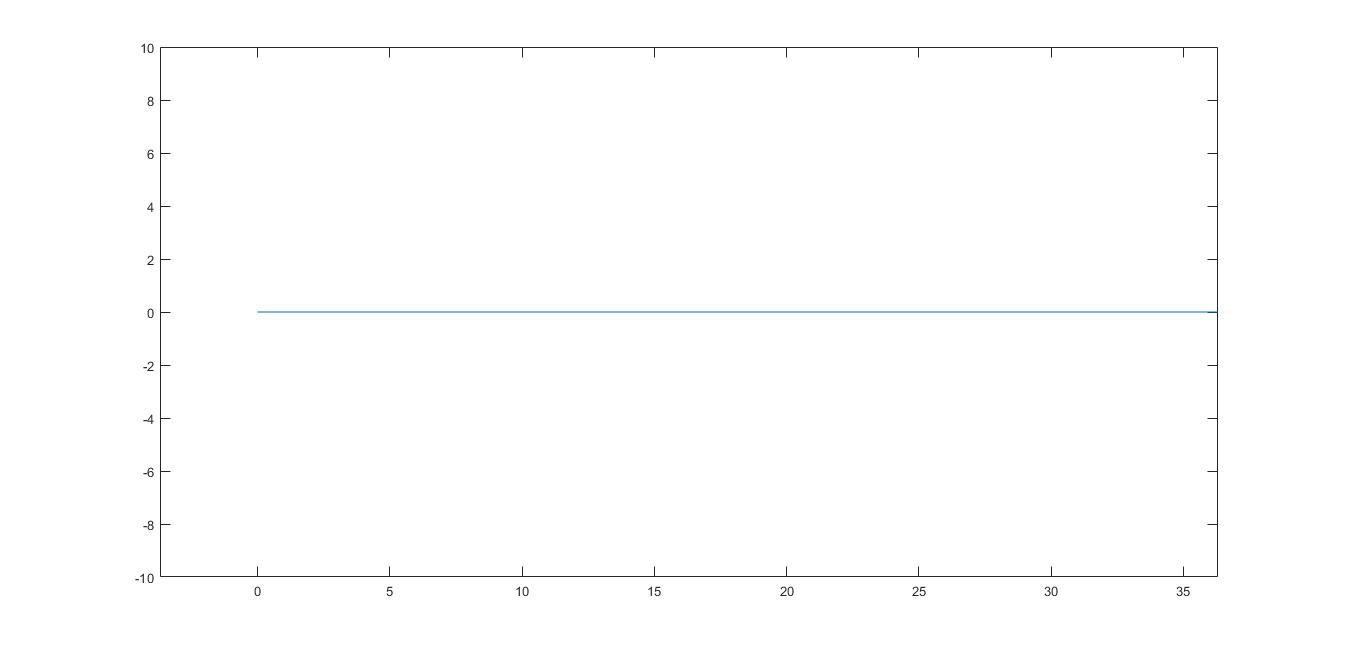
\includegraphics[scale=0.3]{img2.jpg}
\caption{Parte Imaginária - Raíz 2}
\label{fig:real2}
\end{figure}
Para a raíz 2 a parte real será sempre negativa. Além disso, ela não possui parte imaginária para $\alpha>0$. Então, concluímos que a raiz 2 quando $t\rightarrow \infty$ sua contribuição para a resposta tendenderá a zero. 
\\
\\
Raíz  3:
\begin{figure}[H]
\centering
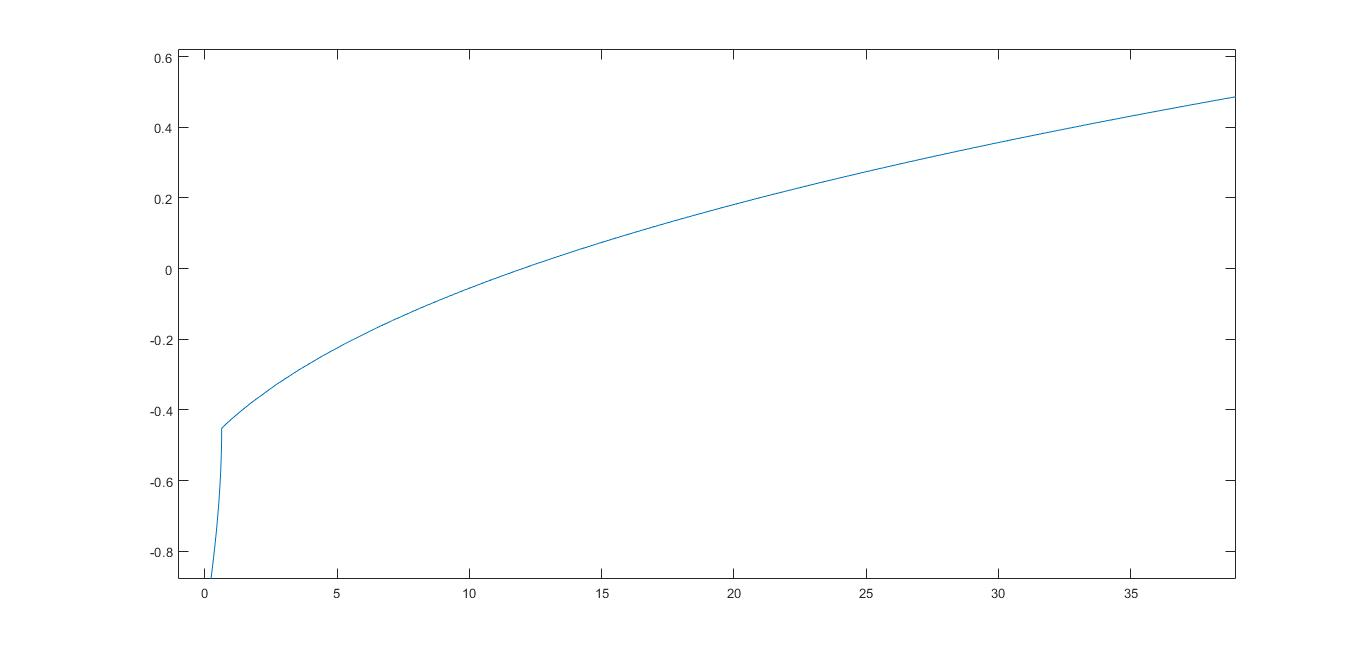
\includegraphics[scale=0.3]{real3.jpg}
\caption{Parte Real - Raíz 3}
\label{fig:real3}
\end{figure}
\begin{figure}[H]
\centering
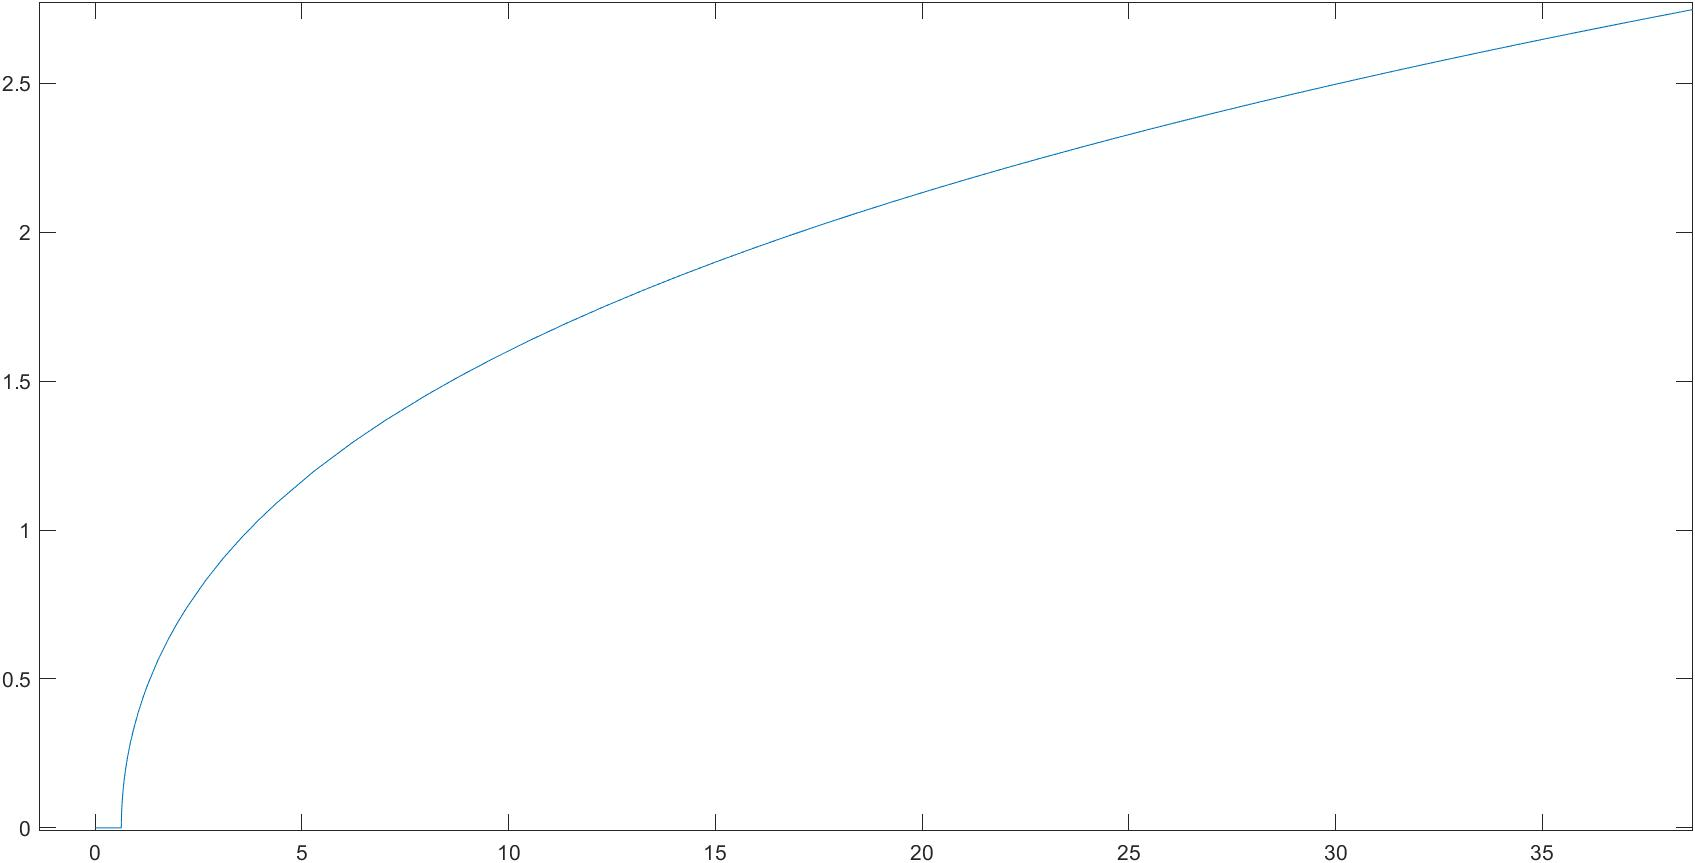
\includegraphics[scale=0.2]{img3.jpg}
\caption{Parte Imaginária - Raíz 3}
\label{fig:real3}
\end{figure}
A raíz 3 terá parte imaginária sempre positiva. Para $0<\alpha<12$ a parte real será negativa, para $\alpha=12$ ela será zero e para $\alpha>12$ ela será positiva. Então, concluímos que a raiz 3 quando $t\rightarrow \infty$ sua contribuição para a resposta de  $0<\alpha<12$ será uma oscilação que tende a zero. Para $\alpha=12$, será uma oscilação que não tende a infinito e também não tende a zero. Já para $\alpha>12$, sua contribuição para resposta será uma oscilação que tende a infinito.

Pelos gráficos, percebemos que a raiz 1 e raiz 3 são números complexos e a raiz 2 é real, pois somente a raiz 2 possui parte imaginária zero para qualquer $\alpha > 0$.
\newline
%%%%%%%%%%%%%%%%%%%%%%%%%%% Escolha do parâmetro a
\subsection{Escolha do parâmetro $\alpha$}
Juntando as contribuições de cada raiz quando $t\rightarrow \infty$, podemos classificar o sistema e dividí-lo em 3 intervalos importantes de acordo com $\alpha$:
\newline
$\alpha \in$ \, [0,12] - Sistema assintoticamente estável, porque sua resposta à entrada zero tende a zero.\newline
$\alpha $ \,\,\,= \,12 \,- Sistema marginalmente estável, porque sua resposta à entrada zero não tende para zero nem diverge para infinito. \newline
$\alpha \in$ [12,$\infty$]\,- Sistema instável, porque sua resposta à entrada zero diverge para o infinito
\newline
\newline
Assim, para realizar as simulações iremos escolher os valores de $\alpha$ como: \newline
$\alpha$1 = 5 \newline 
$\alpha$2 = 12 \newline
$\alpha$3 = 20

Podemos, agora, encontrar a resposta ao degrau unitário de acordo com os 3 valores escolhidos.
%%%%%%%%%%%%%%%%%%%%%%%%%%% Análise das Raízes Encontrando a resposta ...
\subsection{Encontrando a resposta ao degrau unitário}
Usando a Transformada de LaPlace para encontrarmos a resposta ao degrau unitário e utilizando as raízes encontradas no item 1.1:
Sabemos que:
\begin{flalign*}
Y(s) = F(s).H(s)\\
f(t) = u(t), F(s)= \frac{1}{s}
\end{flalign*}

\begin{flalign*}
Y(s) = \frac{1}{s}. \frac{\alpha}{s^3 +4s^2 +3s +\alpha} = \frac{\alpha}{s(s^3 +4s^2 +3s +\alpha)}
\end{flalign*}

\begin{flalign*} 
Y(s) = \frac{A}{s} + \frac{B}{s-r_{1}} + \frac{C}{s-r_{2}} + \frac{D}{s-r_{3}}\\
A = \lim_{s \to 0} s. Y(s) = \lim_{s \to 0} \frac{\alpha}{s^3 +4s^2 +3s +\alpha}= 1
\end{flalign*} 

\begin{flalign*}
B=  \lim_{s \to r_{1}} (s-r_{1}). Y(s) = \lim_{s \to r_{1}} \frac{\alpha}{s(s-r_{2})(s-r_{3})}= \frac{\alpha}{r_{1}(r_{1}-r_{2})(r_{1}-r_{3})}
\end{flalign*}

\begin{flalign*}
C=  \lim_{s \to r_{2}} (s-r_{2}). Y(s) = \lim_{s \to r_{2}} \frac{\alpha}{s(s-r_{1})(s-r_{3})}= \frac{\alpha}{r_{2}(r_{2}-r_{1})(r_{2}-r_{3})}
\end{flalign*}

\begin{flalign*}
D =  \lim_{s \to r_{3}} (s-r_{3}). Y(s) = \lim_{s \to r_{3}}\frac{\alpha}{s(s-r_{1})(s-r_{2})}=\frac{\alpha}{r_{3}(r_{3}-r_{1})(r_{3}-r_{2})}
\end{flalign*}


Então a resposta:
\begin{equation} \label{eqy}
        y(t) = A + B.e^{r_{1}\cdot t} + C.e^{r_{2}\cdot t} +D.e^{r_{3}\cdot t}, t\geq0
\end{equation}
Com os valores de $\alpha$ selecionados, podemos finalmente encontrar a resposta ao degrau unitário para cada um deles, podemos substituir $\alpha$ por 5, 15 e 20 na equação (\ref{eqy}). Utilizando o matlab encontramos:\\
$\alpha$ = 5:
\begin{equation*}
\begin{split}
y(t)= 1- 0.886744881532621862402273\\ e^{-0.22414947600742854037692357t}\cos(1.16513224774005205008t)\\
-0.51583133559630411189e^{-0.224149476007428540376t}\sin(1.1651322477400520500891t))\\
-0.1132551184673781375977263e^{-3.55170104798514291924t}
\end{split}
\end{equation*}

\begin{figure}[H]
\centering
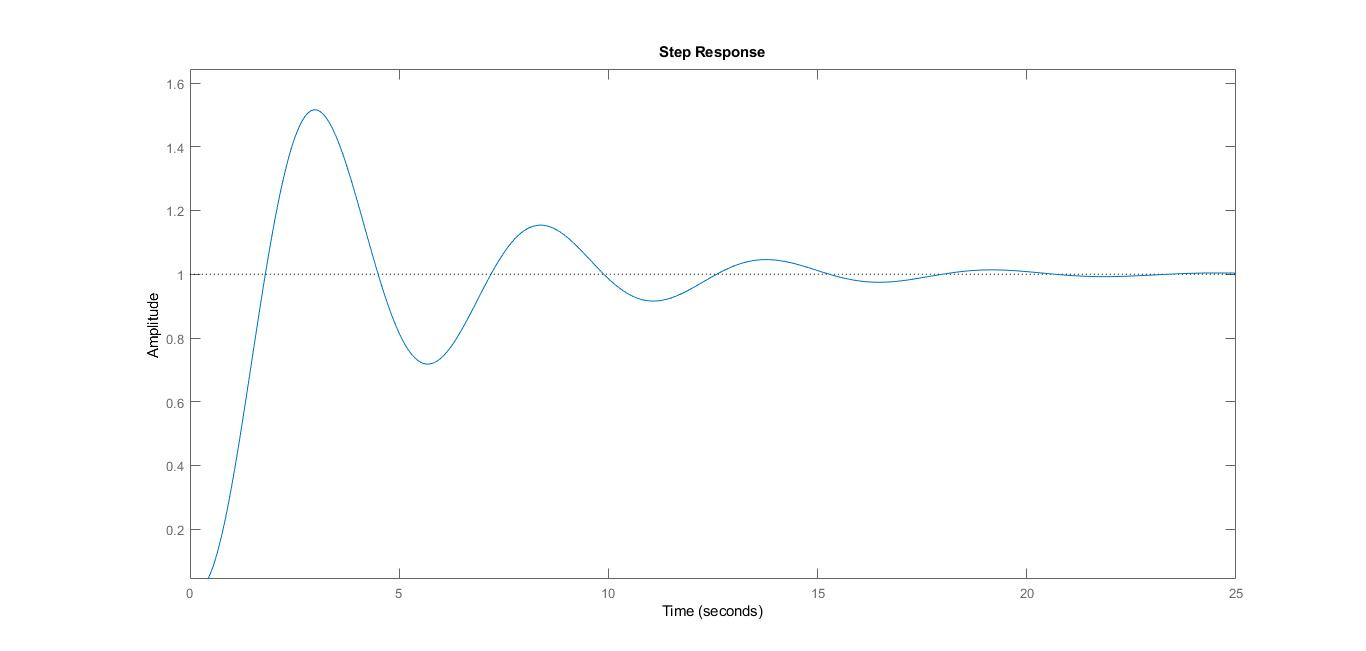
\includegraphics[scale=0.3]{a=5.jpg}
\caption{y(t) para $\alpha$=5}
\label{fig:a=5}
\end{figure}


 $\alpha$ = 12:
\begin{equation*}
y(t) = 1 -\frac{16\cos(\sqrt{3}t) }{19} -\frac{4\sqrt{3}\sin(\sqrt{3}t)}{19}-\frac{3e^{-4t}}{19}
\end{equation*}

\begin{figure}[H]
\centering
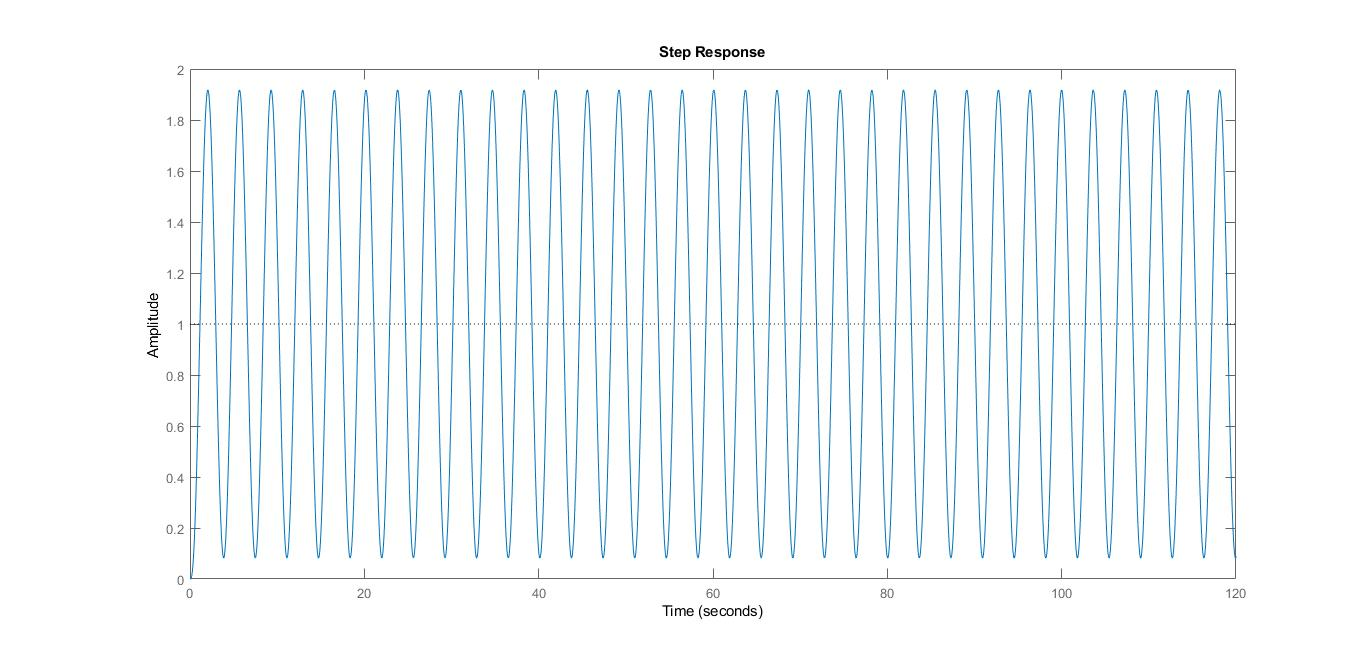
\includegraphics[scale=0.3]{a=12.jpg}
\caption{y(t) para $\alpha$=12}
\label{fig:a=12}
\end{figure}

$\alpha$ = 20:
\begin{equation*}
\begin{split}
y(t) = 1-0.818126001058066915770297787\\
e^{0.1815201528758580502201t}\cos(2.13330961670055972081t)\\
-0.302355188444576174666461861e^{0.18152015287585805022017725t}\sin(2.1333096167005597208188737t) \\
-0.1818739989419330842297022e^{ -4.36304030575171610044035451t}
\end{split}
\end{equation*}

\begin{figure}[H]
\centering
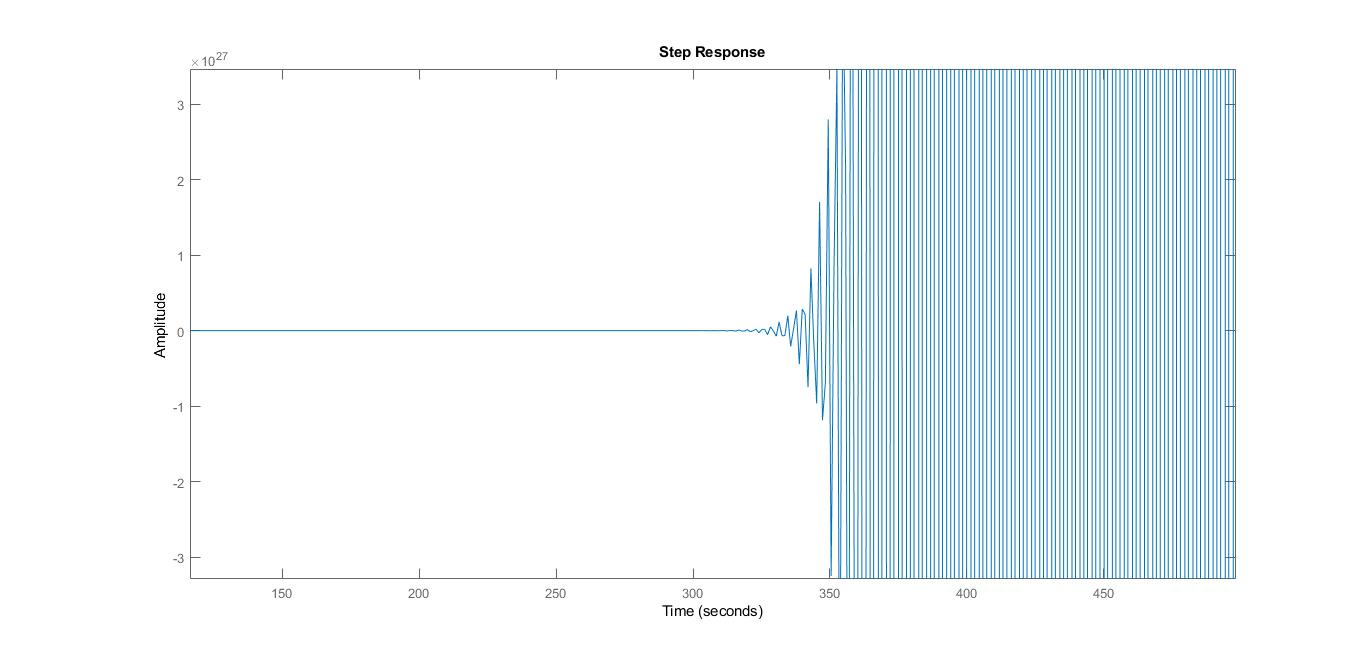
\includegraphics[scale=0.3]{a=20.jpg}
\caption{y(t) para $\alpha$=20}
\label{fig:a=20}
\end{figure}





%%%%%%%%%%%%%%%%%%%%%%%%%%% SEÇÂO 2 %%%%%%%%%%%%%%%%%%%%%%%%%%%%%%%
\section{Expressão da resposta em frequência e Diagrama de Bode}
\subsection{Expressão da resposta em frequência}
Para obtermos a resposta em frequência H(jw), basta fazer s = jw na equação (\ref{eqfunction}):


\begin{equation*}
H(jw) = \frac{\alpha}{(jw)^3 +4(jw)^2 +3jw +\alpha}\\
\end{equation*}
\begin{equation*}
H(jw) = \frac{\alpha}{-jw^3 -4w^2 +3jw +\alpha}\\
\end{equation*}

\begin{equation} \label{jw}
H(jw) = \frac{\alpha}{(-4w^2 +\alpha) +(3w-w^3)j}\\
\end{equation}

\subsection{Analisando os pólos}
Agora iremos analisar o comportamento dos pólo real e o par de pólos complexos para relacionar ao Diagrama de Bode da função de transferência.
Vamos manipular a equação em função das raízes $r_{1}$, $r_{2}$ e $r_{3}$. Como visto anteriormente, para os valores escolhidos de $\alpha$, $r_{2}$ é puramente real e $r_{1}$ e $r_{3}$ são complexas conjugadas. Iremos usar apenas os valores de $\alpha$ = 5 e  $\alpha$ = 12, pois para $\alpha$ = 20 teremos pólos no semiplano direito tornando o sistema instável, sendo que o diagrama de bode só analisa sistemas em regime permanente.
\begin{equation}
\begin{split}
H(s)=\frac{\alpha}{s^3+4s^2+3s+\alpha}
\\
H(s)=\frac{\alpha}{(s-r_{1})(s-r_{2})(s-r_{3})}
\\
H(s)=\frac{\alpha}{-r_{1}.r_{2}.r_{3}} \,.\, \frac{1}{(1-\frac{s}{r_{2}})} \,.\, \frac{1}{(1-\frac{s}{r_{1}}).(1-\frac{s}{r_{3}})}\\
\end{split}
\end{equation}

\noindent Substituindo $\alpha$ por 5 e 12 na equação (\ref{r1}), equação (\ref{r2}) e equação (\ref{r3}):
\noindent\begin{itemize}
\item $\alpha$ = 5: 
    \begin{itemize}
         \item $r_{1}$ = -0.2241 + 1.1651j
         \item $r_{2}$ = -3.5517
         \item $r_{3}$ = -0.2241 - 1.1651j
    \end{itemize}
\end{itemize}


\noindent\begin{itemize}
    \item $\alpha$ = 12:
        \begin{itemize}
            \item $r_{1}$ = 1.7321j
             \item $r_{2}$ = -4
             \item $r_{3}$ = -1.7321j
        \end{itemize}
\end{itemize}


Agora podemos dividir os 3 termos respectivamente em $H_{0}$, $H_{1}$ e $H_{2}$ e analisá-los isoladamente.
\\

%% H0
\begin{itemize}
    \item  \underline{\large{\textbf{H_{0}}}:}
\end{itemize}\\
O termo $H_{0}$ não irá depender de w e por isso se comportará como uma constante que terá o valor em função de $\alpha$. Analisando o denominador através dos valores de $r_{1}$, $r_{2}$ e $r_{3}$ para $\alpha$ = 5 e $\alpha$ = 12 podemos verificar que ele irá será muito próximo de - - $\alpha$.\\ \\
\textit{ {\small
$\alpha$ = 5 : $(-3.5517 + 0.0000j)*(-0.2241 + 1.1651j)*(-0.2241 - 1.1651j) = -4.9997$\\
$\alpha$ = 12 : $(-4.0000 + 0.0000j)*(-0.0000\,\,+ 1.7321j\,)*(-0.0000 - 1.7321j) = -12.0007$ }}\\
Assim, $\frac{\alpha}{-r_{1}.r_{2}.r_{3}}$  $\approx $ 1, Mód(dB) [H0] = 20.log(1) = 0 e Fase[H0] = arctg(0) = 0. Então podemos concluir que o termo H0 não irá afetar o diagrama.
\\ 
%% H1
\begin{itemize}
    \item \underline{\large{\textbf{H_{1}}}:}
\end{itemize}\\
No domínio da frequência o termo $H_{1}$ será dado por $\frac{1}{(1-\frac{jw}{r_{2}})}$ e assim teremos:
\text{Mód(db) = $-20 log\left |1 - \frac{jw}{r_{2}} \right |$} \\
\text{Fase = - arctg($\frac{w}{r_{2}}$)}\\
w $\gg$ $r_{2}$: Fase = -90$^{\circ}$ e Mód(dB) = $-20 log\left |\frac{jw}{r_{2}} \right |$ = $-20 log(\frac{w}{r_{2}})$, inclinação de -20dB/dec \\
w $\ll$ $r_{2}$ : Fase = 0$^{\circ}$\, e Mód(dB) = $-20 \, log(1) \approx 0$ dB \,\,\,\\ 
w = $r_{2}$: Fase = -45$^{\circ}$ e Mód(dB) = 20log$|\frac{1}{1+j}|$ = 20log1 -20log$\sqrt{2}$ $\approx$ -3dB
\\
%% H2
\begin{itemize}
    \item \underline{\large{\textbf{H_{2}}}:}
\end{itemize}

\noindent Analisando o termo $H_{2}$ teremos: 

\begin{equation}
\begin{split}
H_{2}(s)=\frac{1}{(1-\frac{s}{r_{1}}).(1-\frac{s}{r_{3}})} = \frac{r_{1}.r_{3}}{s^2-(r_{1}+r_{3})s+ r_{1}r_{3}}
\end{split}
\end{equation}
Sabemos que para um par de pólos complexos temos a seguinte relação:
\begin{equation}
\begin{split}
\frac{a_{0}}{s^2+a_{1}s+a_{0}} = \frac{w_{n}^2}{s^2+2.\beta.w_{n}.s+w_{n}^2} 
\end{split}
\end{equation}
\textit{ {\small obs.: chamamos o coeficiente de amortercimente($\alpha$) de $\beta$ para não confundir com o parâmeteo $\alpha$ do trabalho}}\\ \\

\noindent Então podemos tirar os valores para a frequência natural e a constante de amortecimento, respectivamente:\\

$w_{n}$ = $\sqrt{r_{1}r_{3}}$ \,\,\, e \,\,\, $\beta$ = $\frac{-(r_{1}r_{3})}{2\sqrt{r_{1}r_{3}}}$  \\ 
\begin{itemize}
    \item  Para $\alpha$ = 5 \, teremos  $w_{n}$ = 1,1865 rad/s e $\beta$ = 0,226 
\end{itemize}
\begin{itemize}
\item Para $\alpha$ = 12 teremos $w_{n}$ = 1,7231 rad/s e $\beta$ = 3,8459  . $10^{-16}$
\end{itemize}

Podemos observar que a constante de amortecimento no $\alpha$ = 5 deu um valor menor do que o $\alpha$ = 12. Assim, o pico de ressonância será acentuado no $\alpha$ = 12 do que no $\alpha$ = 5. Também podemos notar que a constante de amortecimento no $\alpha$ = 12 é muito próximo de 0, logo a frequência máxima será muito próxima da frequência natural. 
\\ \\ 

No domínio da frequência teremos:
\begin{equation}
\begin{split}
H_{2}(jw)=\frac{1}{[1-(\frac{w}{w_{n}})^2] + j.2.\beta (\frac{w}{w_{n}})} = 
H_{2}(jw)=\frac{1}{(1-\frac{w^2}{r_{1}r_{3}}) - \frac{j(r_{1}+r_{3})w}{r_{1}r_{3}}}
\end{split}
\end{equation} \\ \\
Dessa forma, o módulo de $H_{2}$ será dado por:
\begin{equation}
\begin{split}
-20 log\left | (1 - \frac{w^2}{r_{1}r_{3}}) -\frac{ j (r_{1}+r_{3})w}{r_{1}r_{3}}\right |
\end{split}
\end{equation} \\
E para a fase teremos:
\begin{equation}
\begin{split} 
\phase{H_{2}(jw)} = \phase{1} \,\,-\,\,   \phase{
(1-\frac{w^2}{r_{1}r_{3}})-\frac{ j (r_{1}+r_{3})w}{r_{1}r_{3}})}
 \\  
\phase{H_{2}(jw)} = 0 - arctg\begin{bmatrix}\frac{-\frac{(r_{1}+r_{3})w}{r_{1}r_{3}}}{(1-\frac{w^2}{r_{1}r_{3}})}\end{bmatrix}\\
\phase{H_{2}(jw)} = arctg\begin{bmatrix}\frac{(r_{1}+r_{3})w}{r_{1}r_{3}-w^2}\end{bmatrix}
\end{split}
\end{equation} \\
Dessa forma o diagrama deverá apresentar as seguintes características:\\
w $\gg$ $w_{n}$: $\measuredangle$Fase =  -180$^{\circ}$ e Mód(db) = -20log( $\frac{w^2}{r_{1}r_{3}}$) = -40logw + 40log($r_{1}r_{3}$), inclinação de -40dB/dec\\
w $\ll$ $w_{n}$:  Fase = \,\,0$^{\circ}$ \,\,\,\, e Mód(db) = -20log1 $\approx$ 0 dB\\
w = $w_{n}$ : Fase = -90$^{\circ}$ 

\\ \\ \\
\indent Com as magnitudes e fases de cada um dos pólos em função dos intervalos de frequências, podemos realizar uma soma e obter o Diagrama de Bode, que associa fase e magnitude com variação de frequência. Assim:

\begin{equation*}
20log\left | H(jw) \right | = 20log\left | H_{0}(jw) \right | -20log\left | H_{1}(jw) \right | -20log\left | H_{2}(jw) \right |
\end{equation*}
Além disso:
\begin{equation*}
\angle{H(jw)} = \angle{H_{0}(jw)} + \angle{H_{1}(jw)} +\angle{H_{2}(jw)}
\end{equation*}


%%%%%%%%%%%%%%%%%%%%%%%%%%% Analisando o Diagrama de Bode
\subsection{Analisando o Diagrama de Bode}
\begin{figure}[H]
\centering
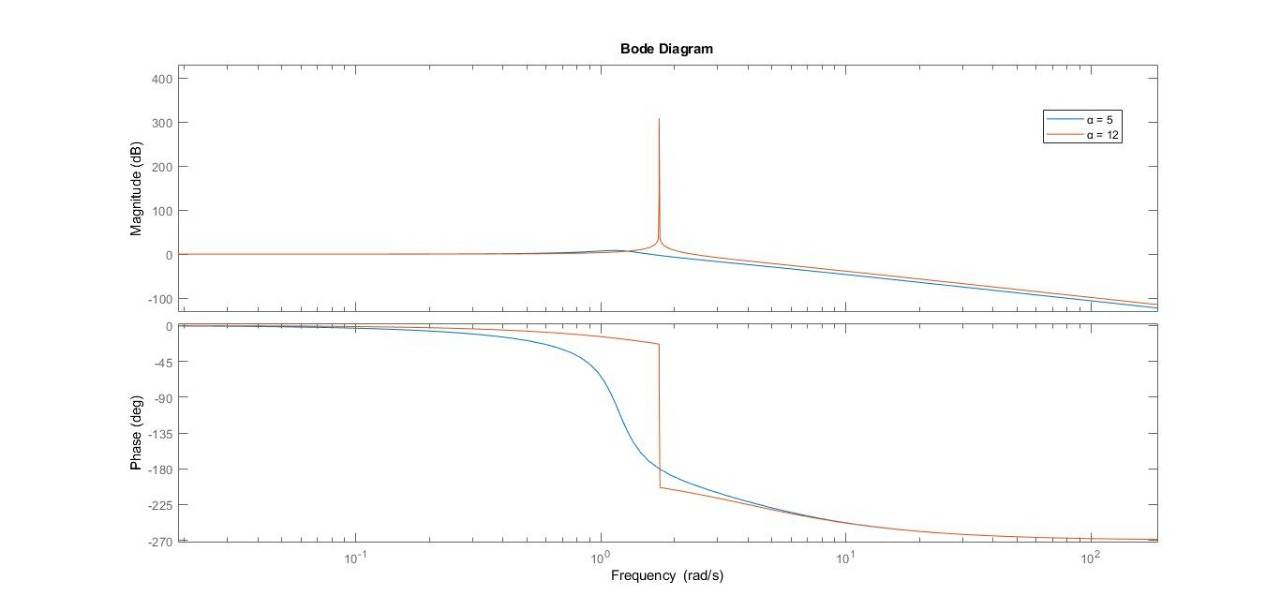
\includegraphics[scale=0.4]{bode.jpg}
\caption{Diagrama de Bode}
\label{fig:diagrama}
\end{figure}
Juntando as informações sobre o comportamento dos pólos no diagrama de bode, podemos entender melhor o que está acontecendo com o diagrama de bode da função de transferência. \newline
\indent Assim, no diagrama de magnitude, podemos perceber que do início até o pico de ressonância, os dois pólos tendem a magnitude zero, então o diagrama de bode de transferência também fica tendendo a zero. \newline
\indent Logo em seguida, temos um pico de ressonância devido ao par de pólos complexos. Como podemos comparar, para $\alpha$ = 5 possui um menor pico do que o $\alpha$ = 12, como calculado já anteriormente, isso se deve ao amortecimento de cada um. No $\alpha$ = 12, a frequência máxima se aproxima da frequência natural por ter um amortecimento próximo de zero, o que explica a frequência de ressonância.\newline
\indent Posteriormente a frequência natural e até ao pólo real, o gráfico cai -40dB/dec devido à contribuição do pólo complexo que também caía a essa taxa.\newline
\indent Do valor do pólo real em diante, o gráfico cai a uma taxa de -60dB/dec devido a contribuição do pólo real que caía a -20dB/dec e ao par de pólos complexos com -40dB/dec.\newline
\indent Observando o gráfico de fase para $\alpha$ = 5, podemos perceber de 0$^{\circ}$ a frequência natural, a contribuição do ângulo é de 0$^{\circ}$ até -90$^{\circ}$, pois inicialmente o par de pólos complexos estava aproximadamente com 0$^{\circ}$ e depois começa a diminuir até chegar em -90$^{\circ}$ no ponto da frequência natural. \newline
\indent Nota-se que no valor da frequência natural do $\alpha$ = 12 o gráfico possui um decaimento muito rápido, se aproximando de uma reta vertical. Isso se deve ao amortecimento do par de pólos complexos ser muito próximo de zero.\newline
\indent Verifica-se uma contribuição tanto do par de pólos complexos e do pólo real no ponto do valor do pólo real dando um valor de fase -225$^{\circ}$, pois o pólo real contribui com -45$^{\circ}$ e o par de pólos complexos com -180$^{\circ}$.  \newline
\indent Também do valor do pólo real ao infinito, o gráfico tende a -270$^{\circ}$ devido a contribuição de -90$^{\circ}$ do pólo real e de -180$^{\circ}$ do par de pólos complexos. \newline
\indent Podemos então concluir que nosso sistema está funcionando como um filtro passa-baixa já que ele irá atenuar as amplitudes de sinais de altas frequências e não irá causar mudanças significativas nas amplitudes de sinais com frequências muito baixas. 






%%%%%%%%%%%%%%%%%%%%%%%%%%% SEÇÂO 3 %%%%%%%%%%%%%%%%%%%%%%%%%%%%%

\section{Resposta em regime permanente para uma entrada senoidal}

%%%%%%%%%%%%%%%%%%%%%%%%%%% Analisando a resposta em função de w
\subsection{Analisando a resposta em função de w}
Iremos fixar o valor de $\alpha$ em 5 e calcular a resposta em regime permanente para uma entrada f(t) = sen(wt). Dessa forma podemos encontrar as seguintes relações para  $\begin{vmatrix}H(jw)\end{vmatrix}$ e $\phase{H(jw)}$ ao utilizar a equacão (\ref{jw}):
\begin{equation}
\begin{split}
\begin{vmatrix} H(jw)
\end{vmatrix}= \frac{5}{\sqrt{w^{6} + 16w^{4} -6w^{^{3}} - 31w^{2} +25}}
\\ \\ 
\phase{H(jw)} = -\arctan (\frac{3w-w^{3}}{5-4w^{2}})
\\
\end{split}
\end{equation}
Para uma entrada senoidal f(t) = A.sen(wt), sabemos que a resposta em regime permanente será dada por Yrp = A.$\begin{vmatrix}H(jw)\end{vmatrix}$.sen(wt + $\phase{H(jw)}$) e por isso nossa resposta em função de w será dada por:
\begin{equation}
\begin{split}
Yrp = \frac{5.sen(wt + \arctan (\frac{3w-w^{3}}{5-4w^{2}}))}{\sqrt{w^{6} + 16w^{4} -6w^{^{3}} - 31w^{2} +25}}
\end{split}
\end{equation}

%%%%%%%%%%%%%%%%%%%%%%%%%%%Escolhendo os valores de w
\subsection{Escolhendo os valores de w}

Precisamos escolher 3 valores de w e para isso vamos analisar o diagrama de bode e verificar como ele se comporta em relação as mudanças de w. Podemos tirar as seguintes conclusões:
\begin{itemize}
    \item Para w $\to$ 0 teremos 20log($\begin{vmatrix}H(jw)\end{vmatrix}$) $\to$ 0 e assim $\begin{vmatrix}H(jw)\end{vmatrix}$ $\to$ 1
\end{itemize}

\begin{itemize}
    \item Para w $\approx $ 1.14 (onde ocorre o pico) teremos
20.log$\begin{vmatrix}H(jw)\end{vmatrix}$ $\approx $ 8,18 e assim
$\begin{vmatrix}H(jw)\end{vmatrix}$ $\approx $ 2,56
\end{itemize}

\begin{itemize}
    \item Para w $\gg$ 1.14 teremos $20\log \begin{vmatrix}H(jw)\end{vmatrix}$ $\to$ -$\infty$ , $\begin{vmatrix}H(jw)\end{vmatrix}$ $\to$ $10^{-\infty }$ e assim $\begin{vmatrix}H(jw)\end{vmatrix}$ $\to$ 0
\end{itemize}
\\

Por isso vamos definir os seguintes valores de w:
\begin{itemize}
    \item w = 0.01
\end{itemize}
\begin{itemize}
    \item w = 1.14
\end{itemize}
\begin{itemize}
    \item w = 20
\end{itemize}


%%%%%%%%%%%%%%%%%%%%%%%%%%% Analisando as respostas
\subsection{Analisando as respostas}
Podemos fazer um gráfico da resposta (em cor azul) e da entrada (em cor cinza) em função do tempo para diferentes valores de w. 
\begin{itemize}
    \item \underline{\large{\textbf{w = 0.01}}:}
\end{itemize}
A entrada será sen($\frac{t}{100}$)\\ \\ 
Simplificando a expressão teremos aproximadamente uma resposta de Yrp = 1.0001 . sen($\frac{t}{100}+0.006$)

A diferença de fase entre os gráficos é tão pequena que só é perceptível se aproximarmos bastante o gráfico, como pode ser visto na segunda imagem. A amplitude será aproximadamente 1 e por isso o gráfico da resposta é muito próximo ao gráfico da entrada. Além disso, podemos perceber que o gráfico encontrado para esse valor de w se assemelha as características que encontramos no Diagrama de Bode, para valores de w $<$ 1.14 rad/s temos uma amplitude próxima de 1 e a fase próxima de zero.

\begin{figure}[H]
\centering
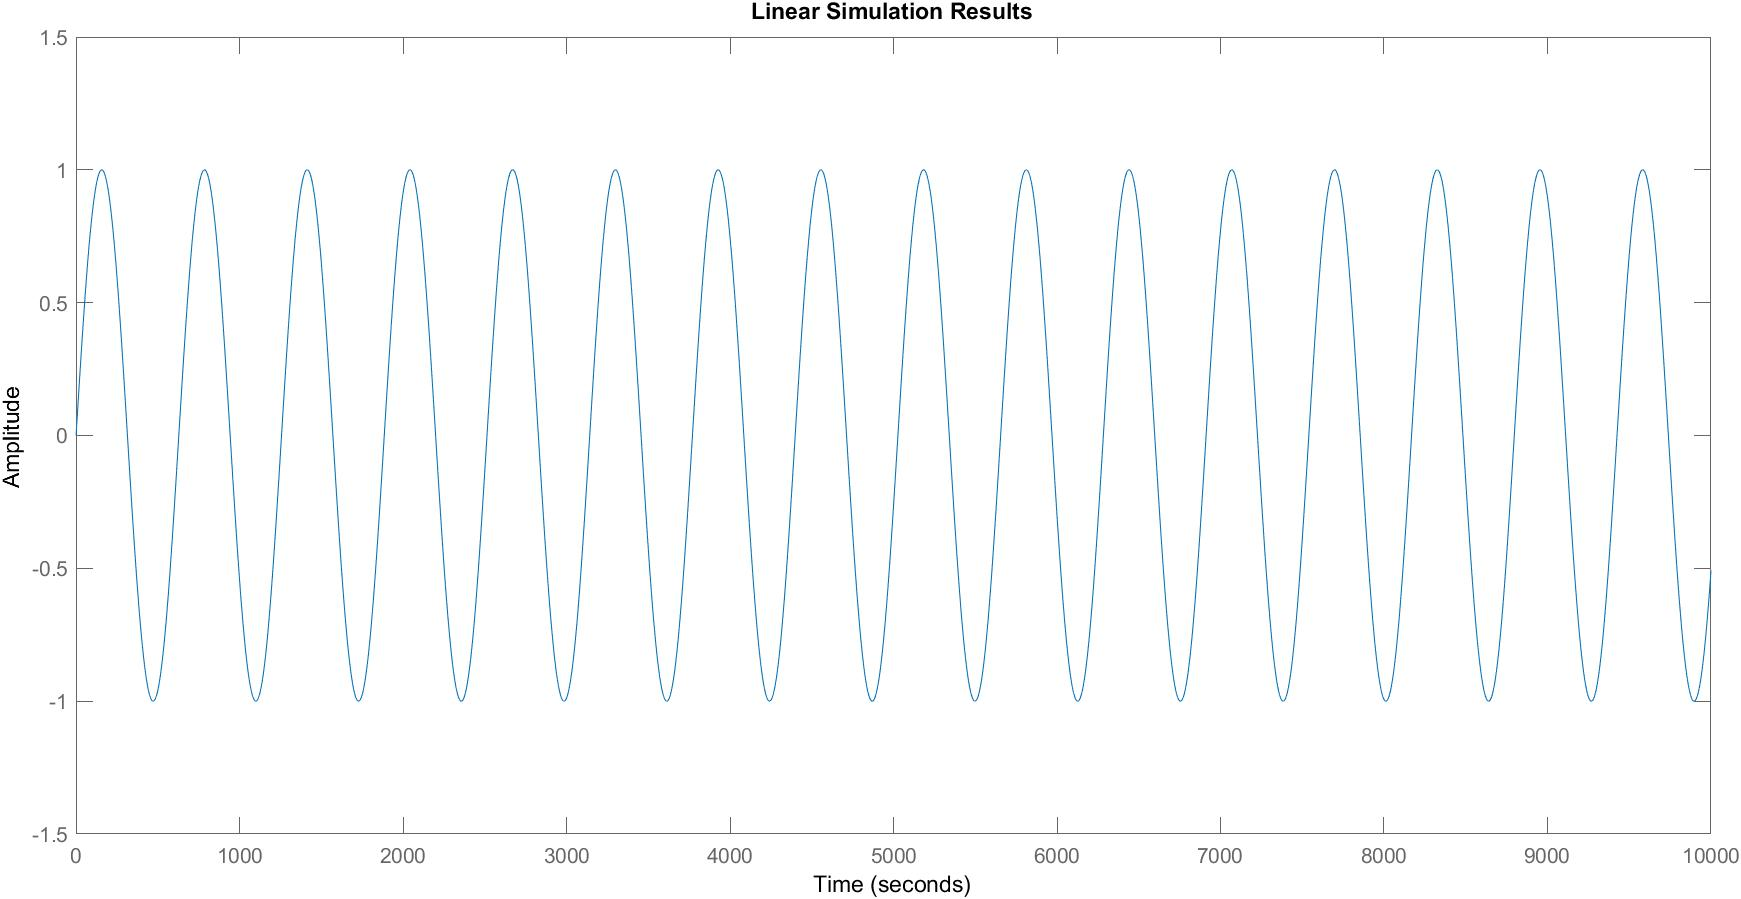
\includegraphics[scale=0.2]{w001.jpg}
\caption{w = 0.01}
\label{fig:diagrama}
\end{figure}

\begin{figure}[H]
\centering
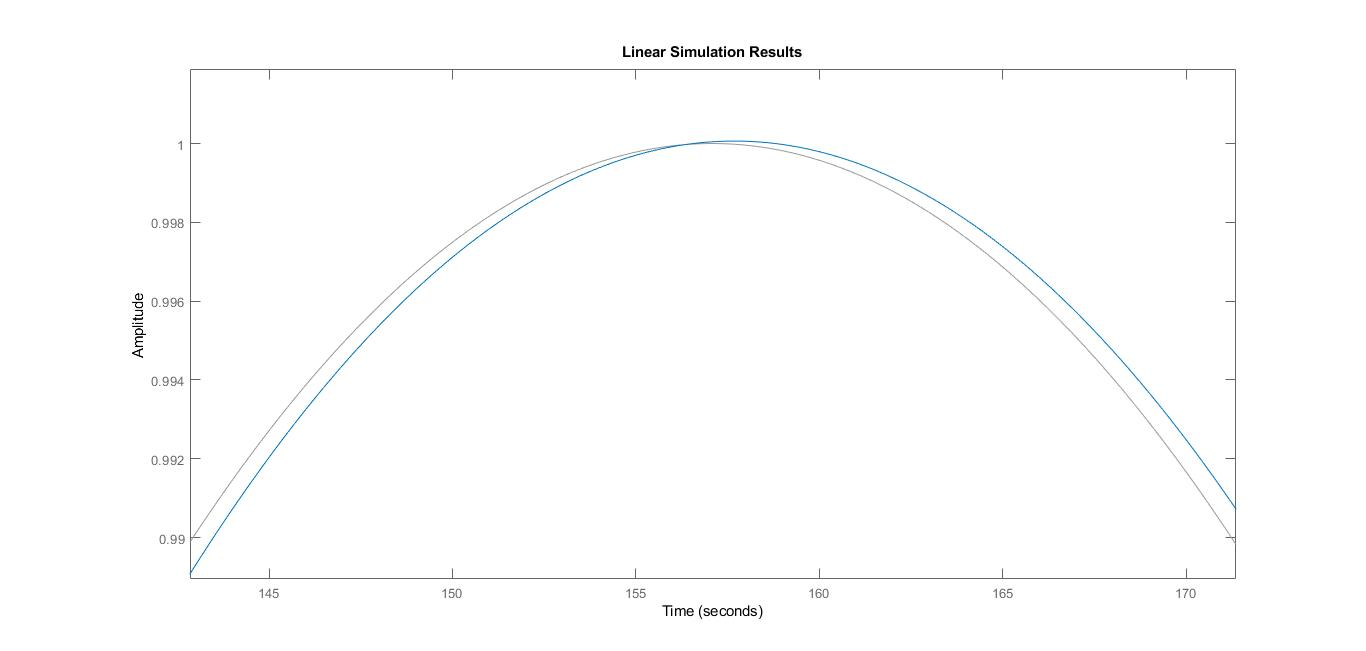
\includegraphics[scale=0.3]{001.jpg}
\caption{w = 0.01 com aproximação}
\label{fig:diagrama}
\end{figure}

\begin{itemize}
    \item \underline{\large{\textbf{w = 1.14}}:}
\end{itemize}
\noindent
A entrada será sen(1.14t)\\
Simplificando a expressão teremos aproximadamente uma resposta de Yrp = 2.2269sen(1.14t-1.4688) 

Também podemos perceber que se assemelha as características do gráfico do Diagrama de Bode. Pelos cálculos realizados anteriormente, esse valor de w nos dá a maior amplitude possível para a resposta e a partir desse valor ela passará a diminuir e tender a zero. Além disso, temos um atraso de aproximadamente 84,15$^{\circ}$, o que faz sentido já que na maior amplitude a fase deveria ser próxima à 90$^{\circ}$. 

\begin{figure}[H]
\centering
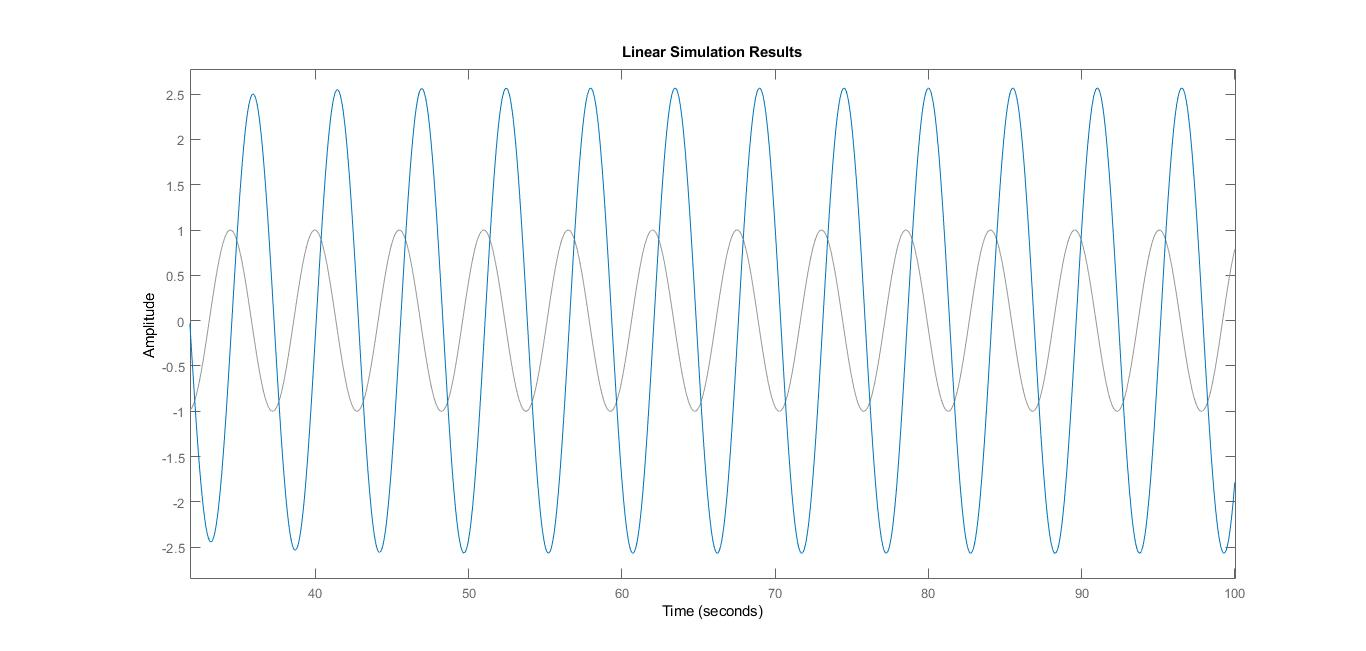
\includegraphics[scale=0.3]{w114.jpg}
\caption{w = 1.14}
\label{fig:diagrama}
\end{figure}

\begin{itemize}
    \item \underline{\large{\textbf{w = 20}}:}
\end{itemize}
A entrada será sen(20t)\\
Simplificando a expressão teremos aproximadamente uma resposta de Yrp = 0.00061314 sen(20t + 1.3726)

\begin{figure}[H]
\centering
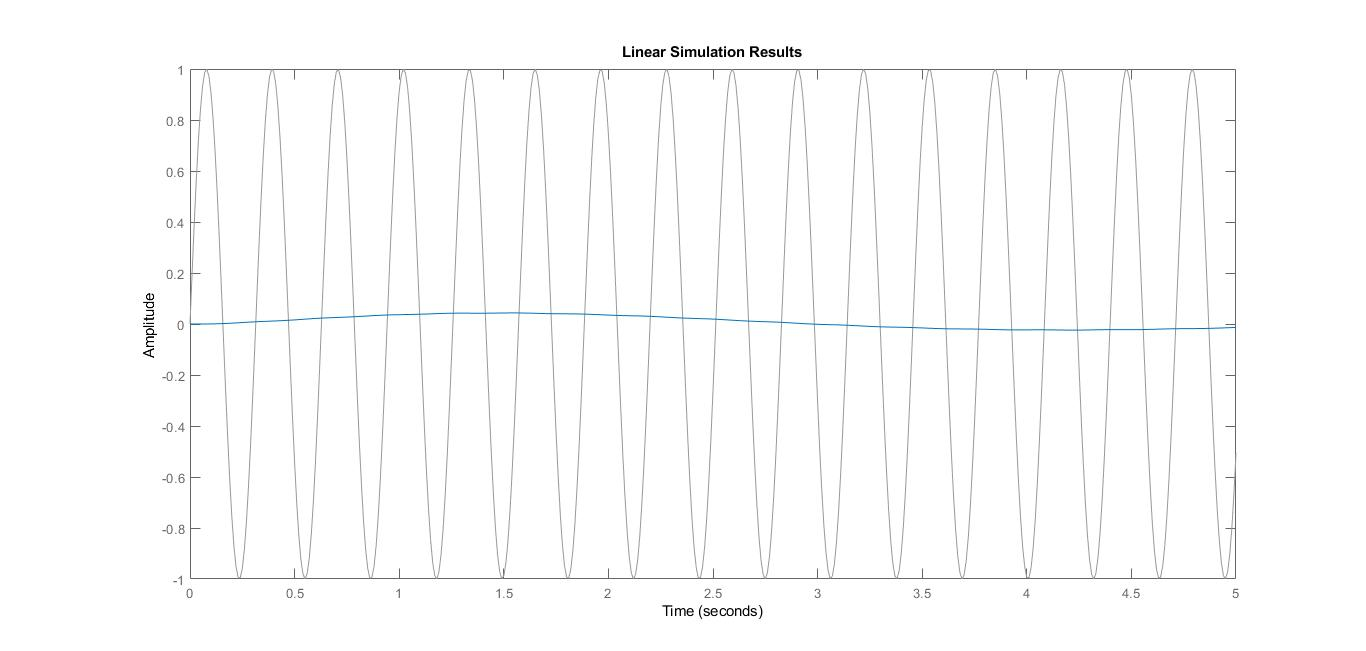
\includegraphics[scale=0.3]{w20.jpg}
\caption{w = 20}
\label{fig:diagrama}
\end{figure}

Como podemos perceber para valores de w $>$ 1.14, o gráfico da resposta possui uma amplitude quase nula, tornando-se mais difícil observar a diferença de fase. Porém, conforme aumentamos o valor de w, maior é a diferença de fase até tender a -270$^\circ$. Como já esperado pelo o que analisamos no Diagrama de Bode.

%%%%%%%%%%%%%%%%%%%%%%%%%%% SEÇÂO 4 %%%%%%%%%%%%%%%%%%%%%%%%%%%%%%%
\section{Resposta a entrada de uma onda quadrada}
\subsection{Encontrando a Série de Fourier}
Utilizando a onda quadrada gerada pelo Matlab, como pode ser observado abaixo:

\begin{figure}[H]
\centering
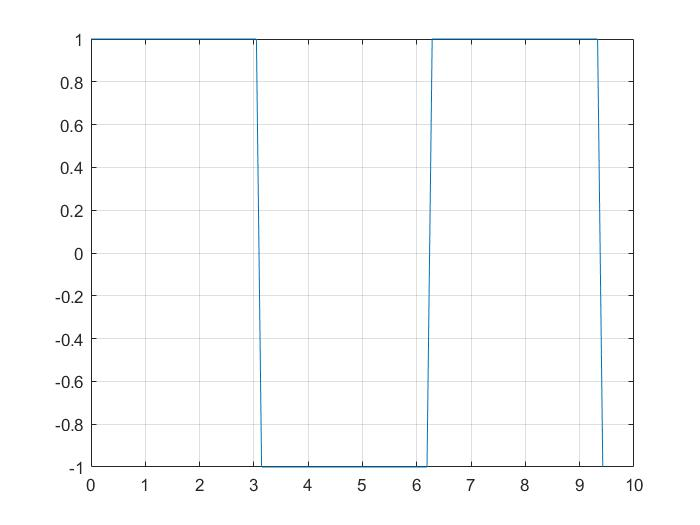
\includegraphics[scale=0.4]{squarewave.jpg}
\caption{Onda quadrada gerada pelo Matlab}
\label{fig:diagrama}
\end{figure}

Por meio dessa onda, podemos achar sua Série de Fourier, sabendo que:
\begin{equation}
f(t) = a_{0} +\sum_{n =1}^{\infty} (a_{n}\cos (nw_{0}t) +b_{n}\sin (nw_{0}t))
\end{equation}

\begin{equation}
    T= 2\pi
\end{equation}
 então:
\begin{equation}
    w_{0} = \frac{2\pi}{T} = 1 
\end{equation}

\begin{equation}
   a_{0} = \frac{1}{T}\int_{t_{0}}^{t_{0}+T}f(t)dt = \frac{1}{2\pi}(\int_{0}^{\pi}dt -\int_{\pi}^{2\pi}dt) = 0
\end{equation}

\begin{equation}
a_{n} = \frac{2}{T}\int_{t_{0}}^{t_{0} +T} f(t)\cos (nw_{0}t)dt = \frac{1}{\pi}[\int_{0}^{\pi}\cos (nt)dt -\int_{\pi}^{2\pi}\cos (nt)dt] = 0
\end{equation}

\begin{equation}
b_{n} = \frac{2}{T}\int_{t_{0}}^{t_{0} +T} f(t)\sin (nw_{0}t)dt = \frac{1}{\pi}[\int_{0}^{\pi}\sin  (nt)dt -\int_{\pi}^{2\pi}\sin (nt)dt] = \frac{1}{n\pi}[2-2\cos (n\pi)]
\end{equation}
Logo, a Série de Fourier fica da forma:
\begin{equation}
    f(t) =\sum_{n=1}^{\infty} \frac{1}{n\pi}[2-2\cos(n\pi)]\sin(nt)
\end{equation}
%%%%%%%%%%%%%%%%%%%%%%%%%%% Somas truncadas
\subsection{Somas truncadas}
Analisando a equação encontrada para a série de fourier, vemos que ela cresce com o termo 1/n fazendo com que os termos com n muito grande sejam pouco significativos e assim tornando necessário a soma de um número muito grande de termos para se chegar ao gráfico original. Como temos um termo $[2-2\cos(n\pi)]$, podemos ver que todos os termos isolados com n par serão nulos e por isso somente os termos com n ímpar irão importar.\\
\indent No primeiro gráfico escolhemos uma soma que vai de n=1 até n=5.Nele, as curvas amarela, roxo e verde representam os gráficos isolados para n=1, n=3 e n=5. Além disso, a curva vermelha representa a soma truncada desses termos e a curva azul mostra a onda quadrada original.
\begin{figure}[H]
\centering
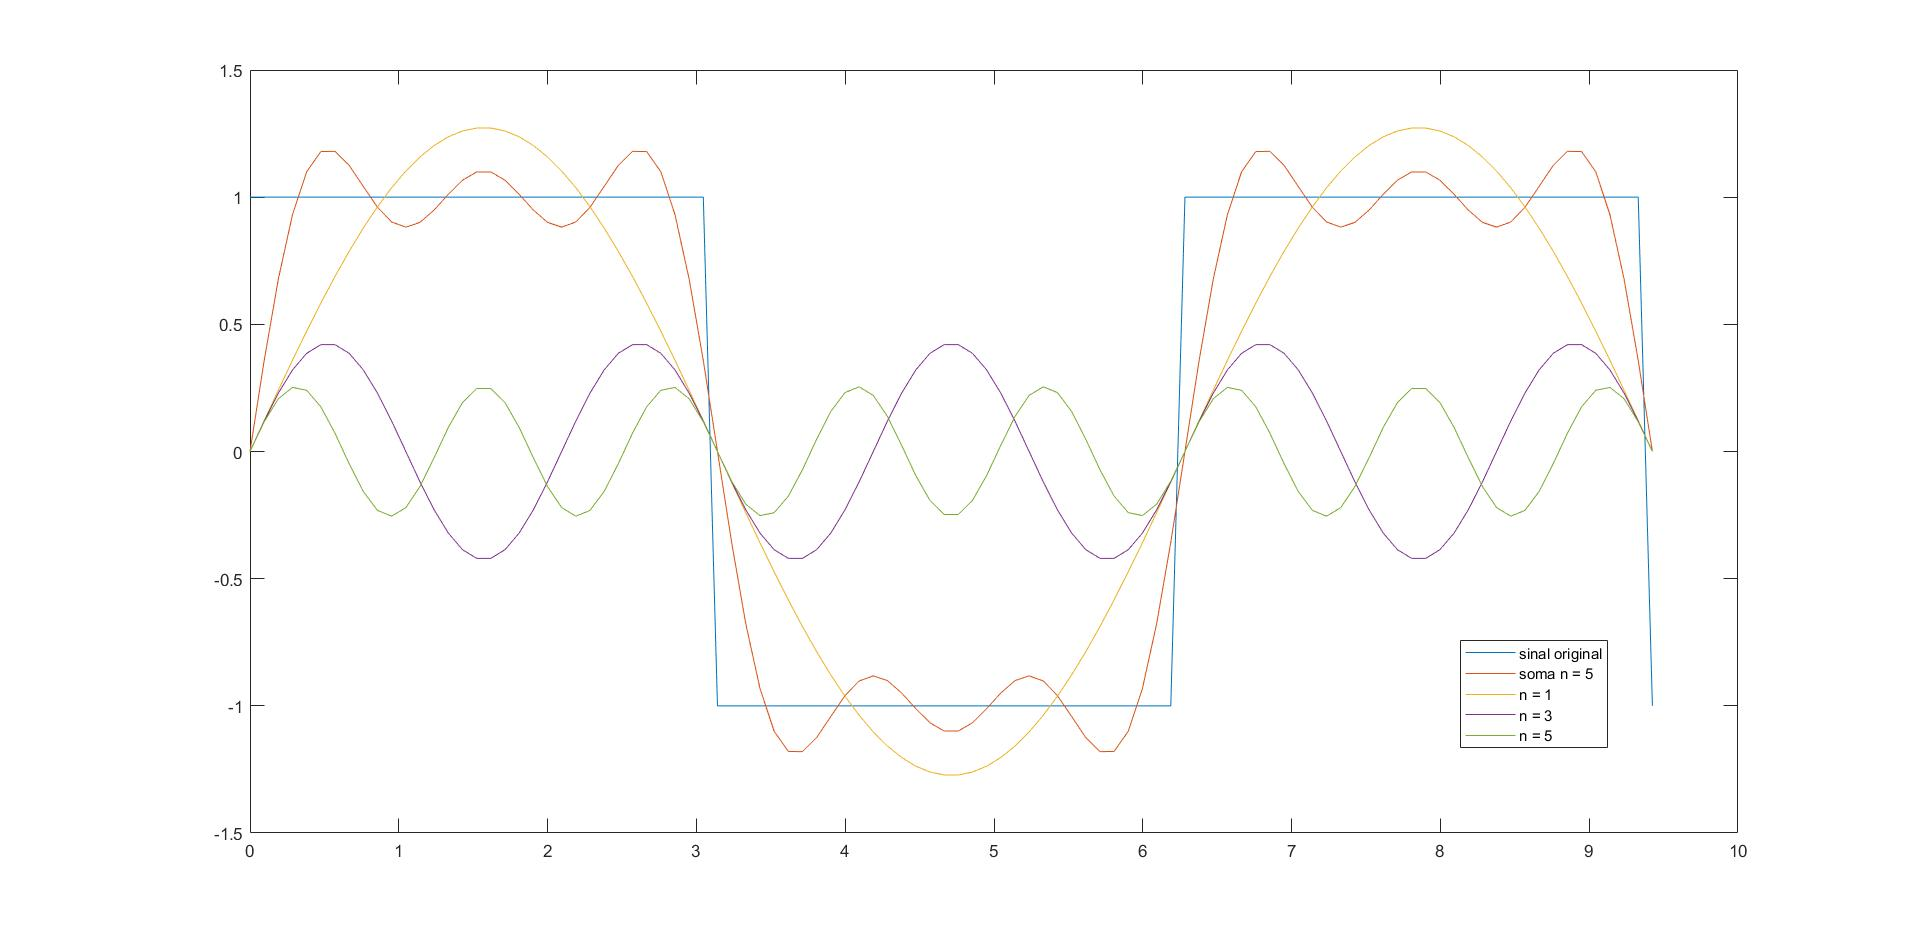
\includegraphics[scale=0.25]{n=5.jpg}
\caption{n=5}
\label{fig:n=5}
\end{figure}

Agora temos a soma para n=15. A curva azul representa a soma truncada desses 9 termos e as outras curvas representam os gráficos isolados de n = 1,3,5,7,9,11,13,15.
\begin{figure}[H]
\centering
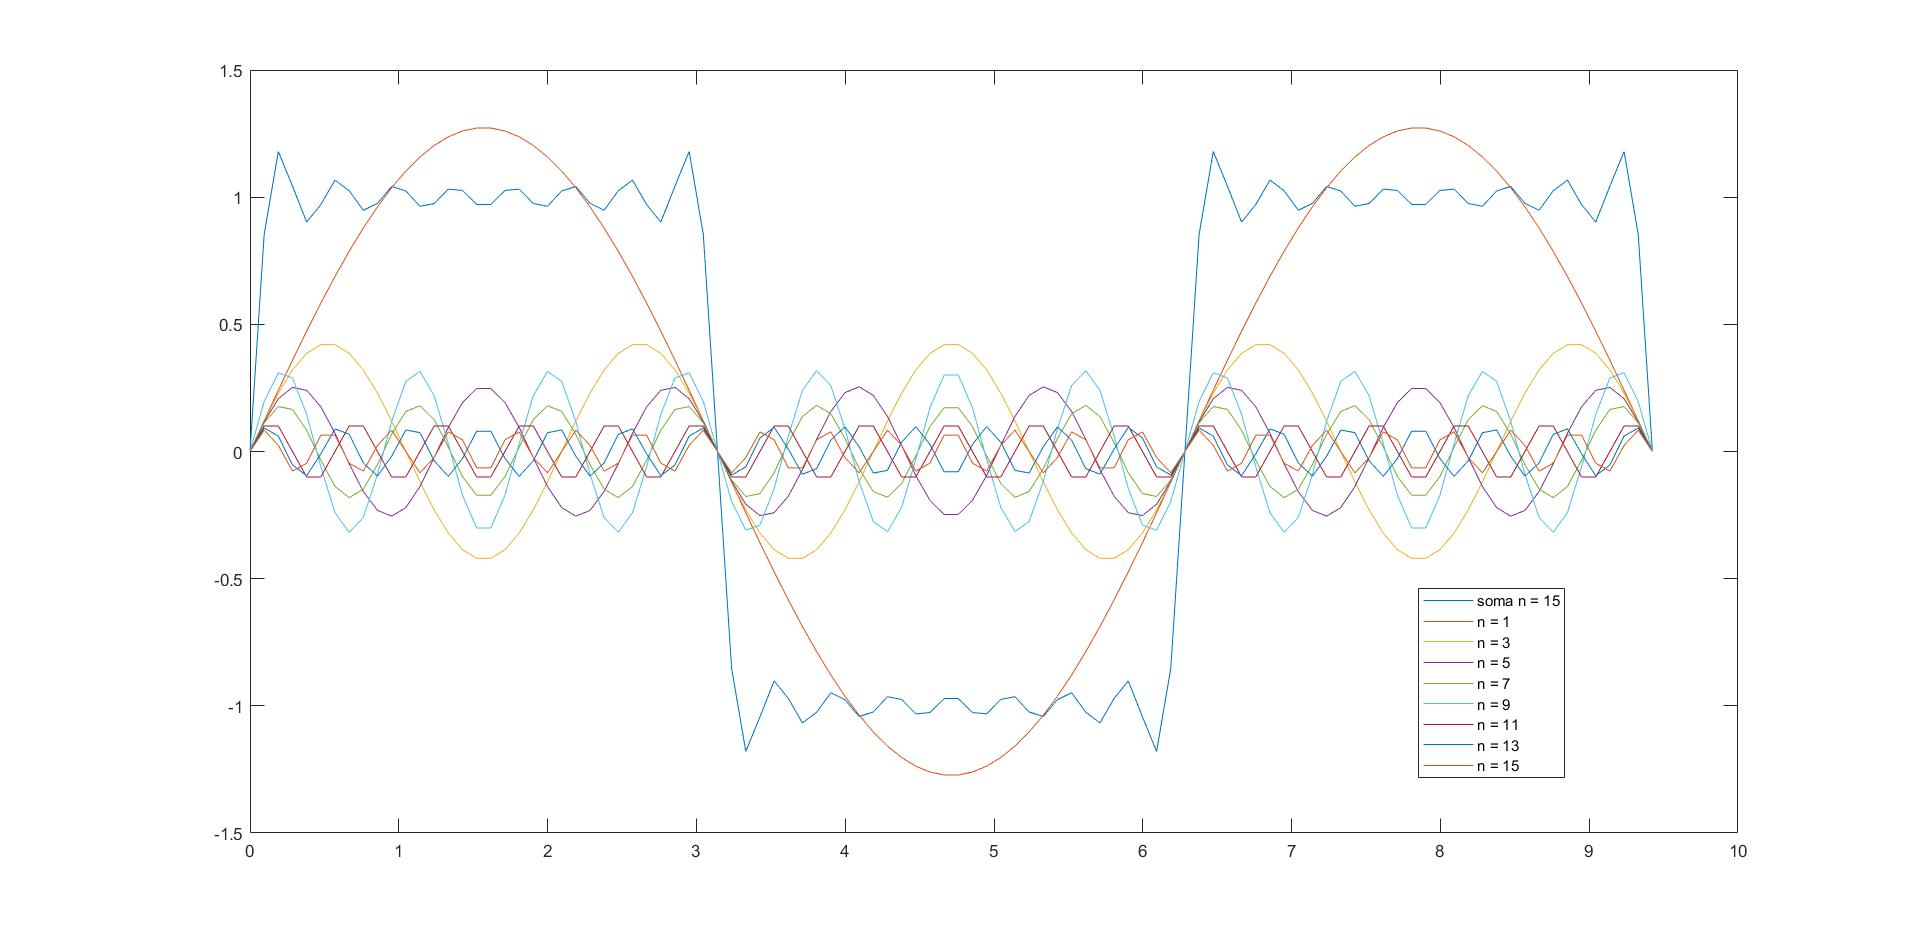
\includegraphics[scale=0.25]{n=15.jpg}
\caption{n=15}
\label{fig:n=15}
\end{figure}

Comparando com o gráfico original vemos que o somatória com n=15 se aproxima bem mais do esperado do que o somatório com n=5. Porém ainda ele ainda possui diferenças muito perceptíveis o que nos leva a deduzir que para chegar em um grádico realmente fiel ao original iríamos precisar de uma soma com um n muito maior.
\begin{figure}[H]
\centering
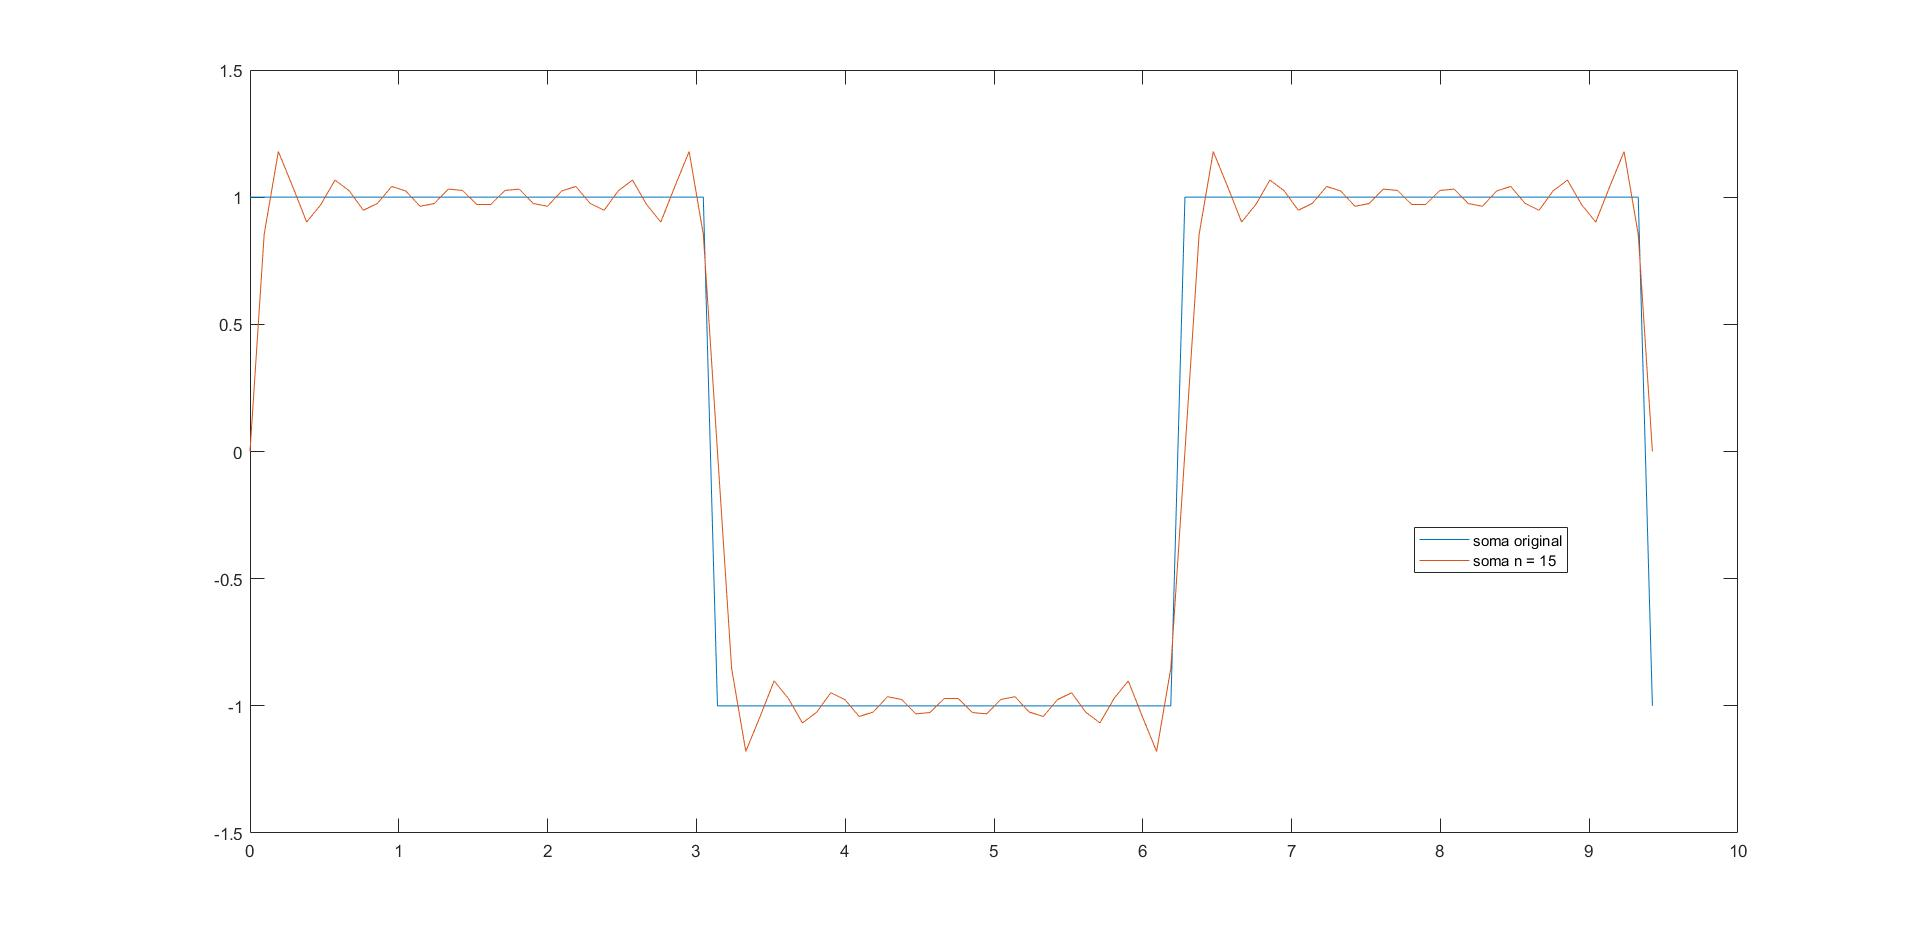
\includegraphics[scale=0.25]{n=15somaoriginal.jpg}
\caption{n=15 e curva original}
\label{fig:n=15 e curva original}
\end{figure}

%%%%%%%%%%%%%%%%%%%%%%%%%%% Analisando as respostas
\subsection{Analisando as respostas}

Vamos fixar o valor de alfa em $\alpha = 12$ e calcular a resposta do sistema às entradas da nossa série escolhida para n=5 e n=15.

\begin{figure}[H]
\flushleft
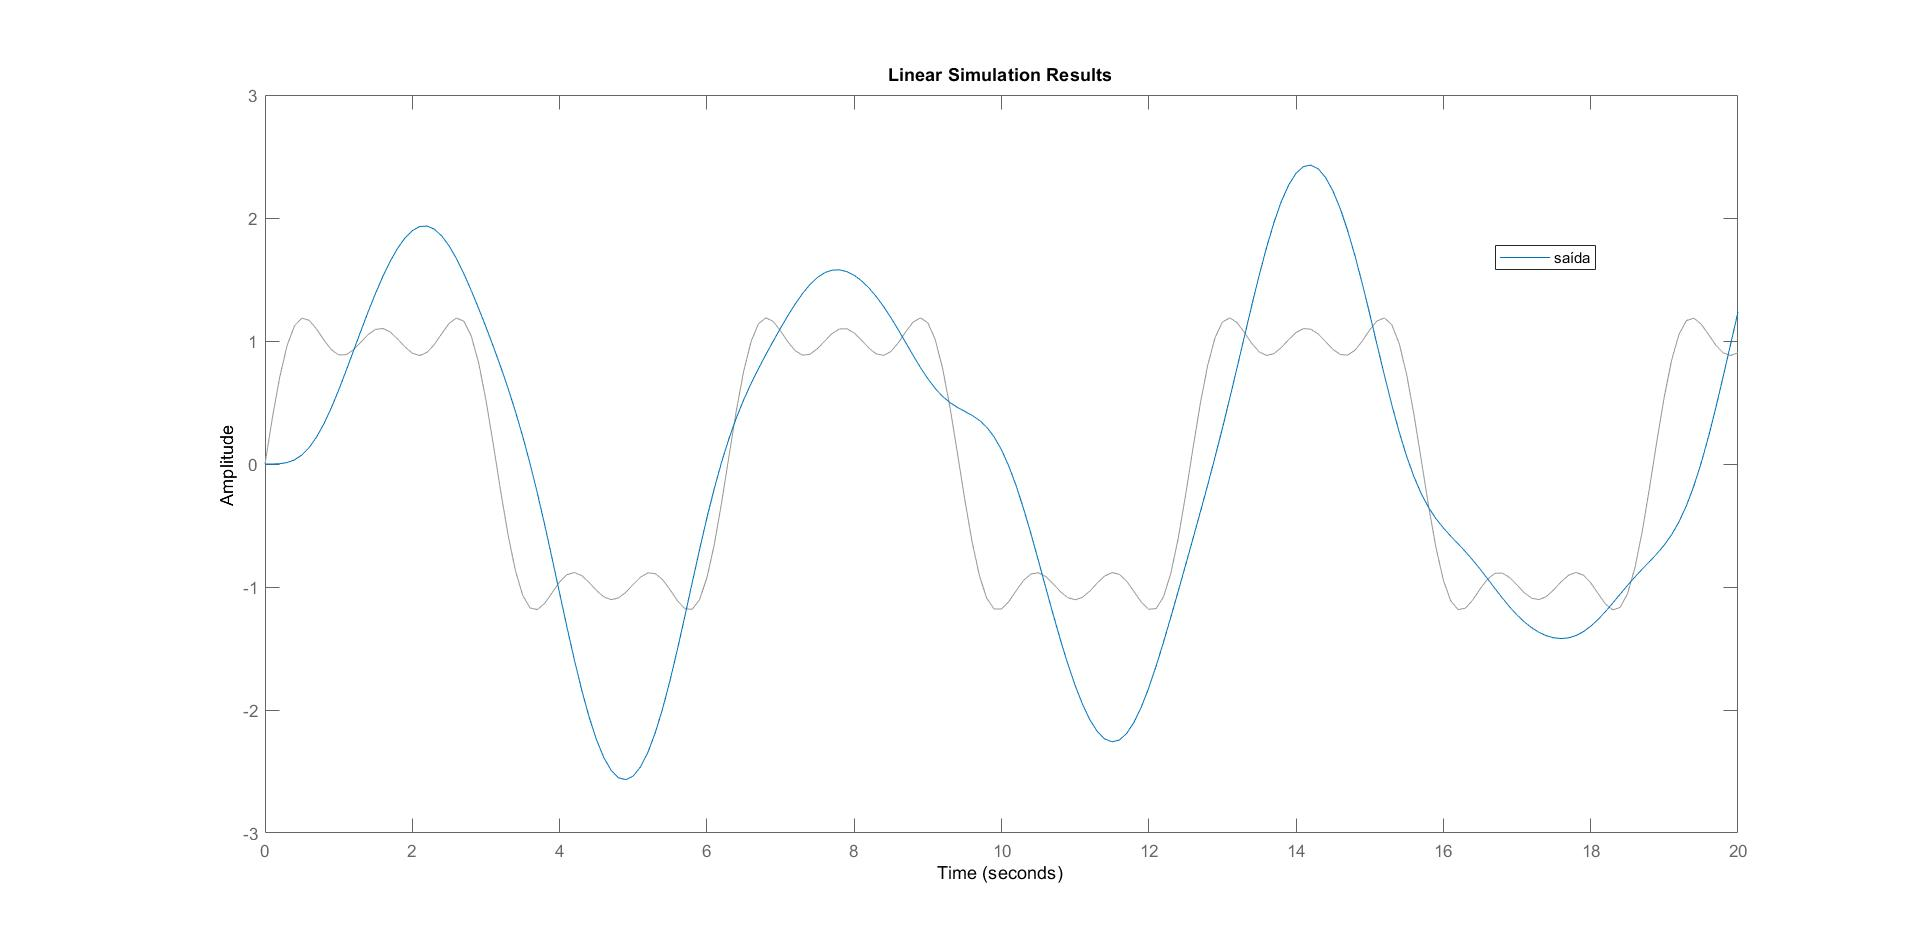
\includegraphics[scale=0.25]{alfa=12n=5.jpg}
\caption{resposta para n=5}
\label{fig:n=15 e curva original}
\end{figure}

\begin{figure}[H]
\flushleft
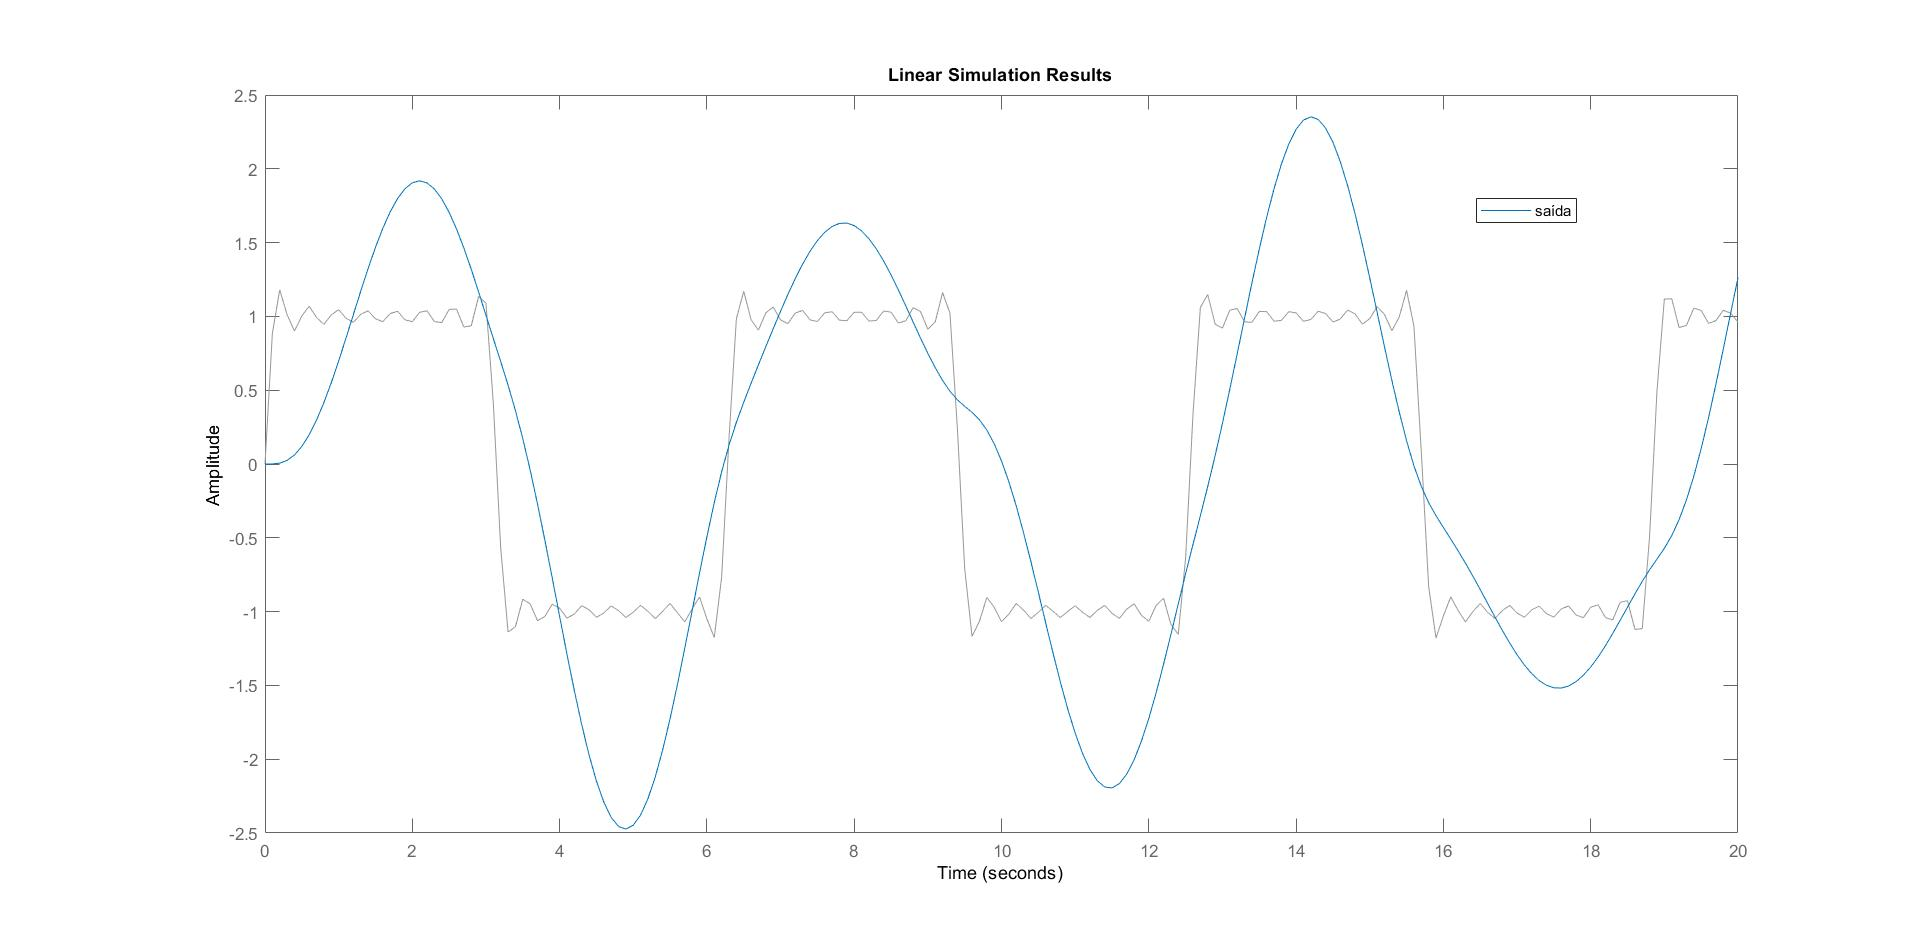
\includegraphics[scale=0.25]{alfa=12n=15.jpg}
\caption{resposta para n=15}
\label{fig:n=15 e curva original}
\end{figure}

Pelos gráficos vemos claramente que apesar dos períodos estarem bem próximos, as amplitudes divergem bastante do gráfico esperado. Porém, como vimos na terceira questão, isso era esperado já que em nosso sistema entradas com frequências próximas a zero terão respostas não-atenuadas, entradas com frequências muito próximas a 1.7231 terão a amplitude de suas respostas amplificadas e respostas com frequências muito grandes terão a amplitude de suas respostas muito atenuadas. Isso caracteriza um filtro passa-baixa.\\
\indent Para verificar este processo vamos analisar o que ocorre com a resposta se agora considerarmos como entrada uma outra onda quadrada de período 200$\pi$ ($w_{0}$ = 0.01 rad/s)
\begin{figure}[H]
\centering
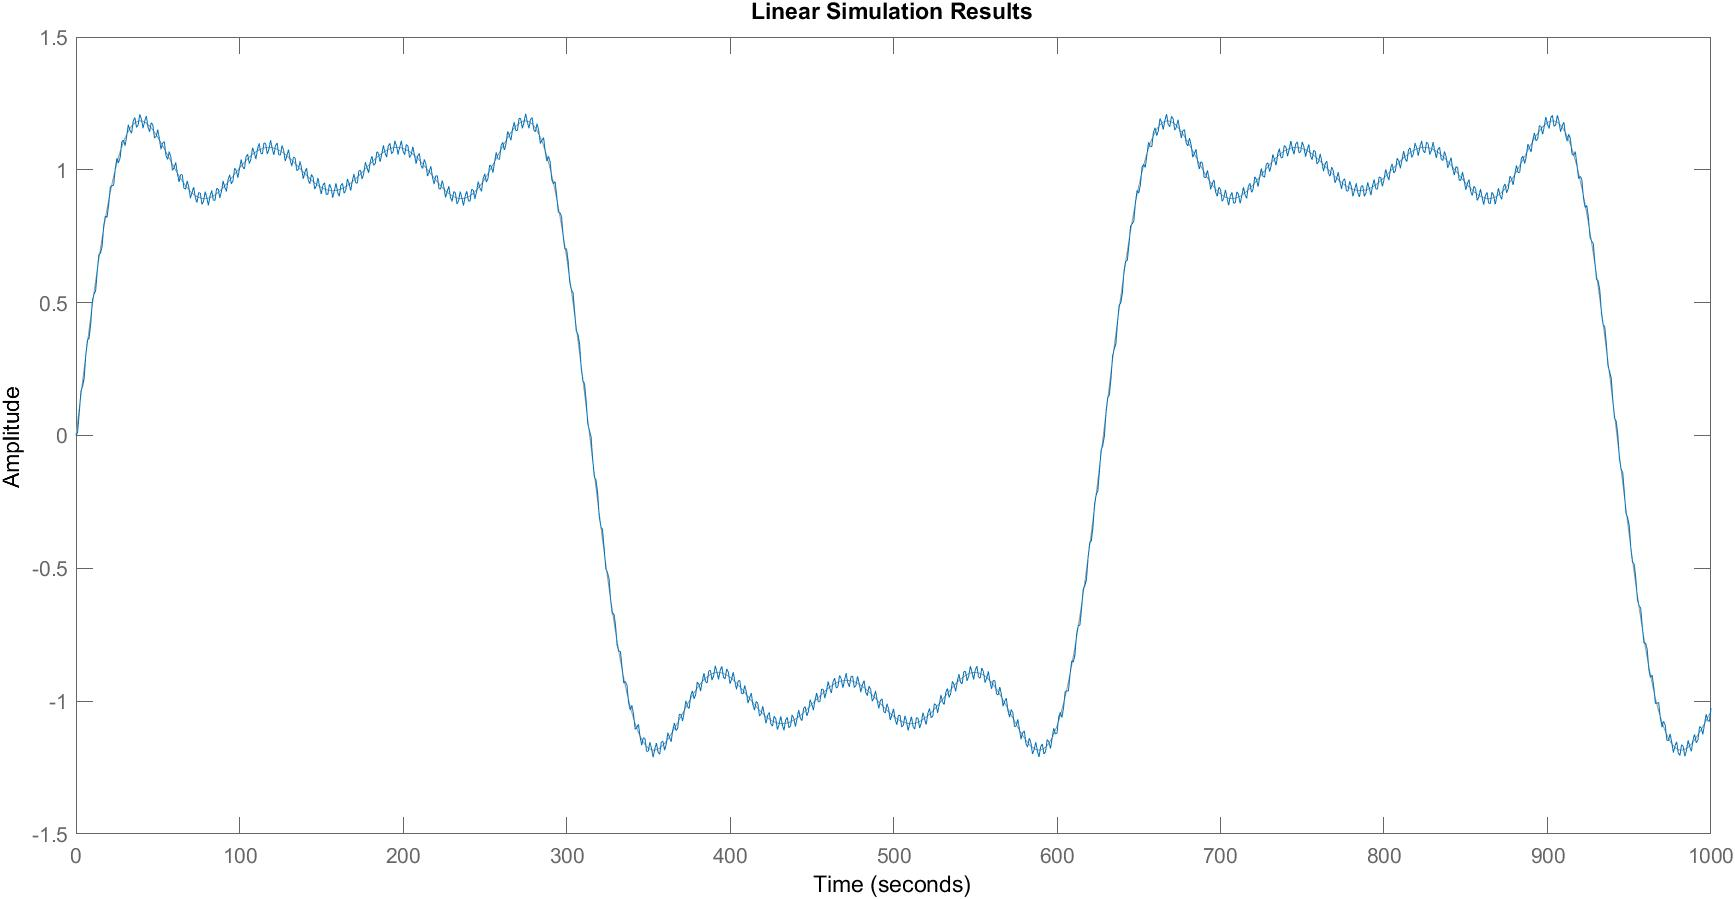
\includegraphics[scale=0.23]{w001n7a12.jpg}
\caption{resposta para n=7}
\label{fig:n=7 e curva original}
\end{figure}
Com esse gráfico podemos ver claramente que a resposta está muito próxima da entrada, confirmando o modelo esperado. O nosso sistema funciona como um filtro passa-baixa  e por isso ter uma frequência muito baixa (0.01) explica a semelhança da saída à entrada escolhida.

%%%%%%%%%%%%%%%%%%%%%%%%%%% SEÇÂO 5 %%%%%%%%%%%%%%%%%%%%%%%%%%%%%%%
\section{Sistema que apresente uma função de transferência entre entrada e saída análoga ao estudado}
O sistema em questão estudado representa um controle proporcional de posição de um motor de corrente contínua modelado como $3^{\circ}$ ordem. Esse pode ser interpretado por um diagrama de blocos do sistema de controle térmico.

\begin{figure}[H]
\centering
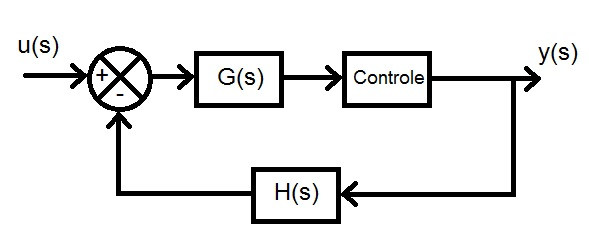
\includegraphics[scale=0.7]{diagrama.jpg}
\caption{Diagrama de bloco}
\label{fig:diagrama}
\end{figure}

 A figura acima pode ser interpretada como G(s) sendo a função de transferência, calculada a partir do parâmetros térmicos, o bloco seguinte é a parte de controle e H(s) é o "feedback", isto é, o retorno do sistema responsável por fornecer informações sobre a saída Y(s). Assim sendo, u(s) funciona como um parâmetro de referência da posição ("Set Point") e o H(s) seria o sensor de posição para comparar a posição de saída Y(s) com a posição u(s).

 Esse controle da posição u(s) ("Set Point") com a posição de saída Y(s) utiliza o desvio, ou seja, a diferença entre o valor esperado de uma variável de processo e seu valor medido por meio de um transdutor.

\end{document}

